% Modified for use with JCC - Madhusudan Singh Copyright (C) (2012). All rights reserved.
\documentclass[12pt]{article}

\setlength{\oddsidemargin}{0in}  %left margin position, reference is one inch
\setlength{\textwidth}{6.5in}    %width of text=8.5-1in-1in for margin
\setlength{\topmargin}{-0.5in}    %reference is at 1.5in, -.5in gives a start of about 1in from top
\setlength{\textheight}{9in}     %length of text=11in-1in-1in (top and bot. marg.) 
\newenvironment{wileykeywords}{\textsf{Keywords:}\hspace{\stretch{1}}}{\hspace{\stretch{1}}\rule{1ex}{1ex}}

\usepackage{amsmath,amssymb}
\usepackage{graphicx}% Include figure files
%\usepackage{caption}
\usepackage{color}% Include colors for document elements
\usepackage{dcolumn}% Align table columns on decimal point
\usepackage{bm}% bold math
\usepackage[numbers,super,comma,sort&compress]{natbib}
%\usepackage[nolists, nomarkers, figuresfirst]{endfloat}

\definecolor{background-color}{gray}{0.98}

\title{Coupling finite and boundary element methods to solve the Poisson-Boltzmann equation for electrostatics in molecular solvation}
\author{Author A\thanks{Department of Biology, University 1, ...}, Author B\thanks{Department of Chemistry, University 2, ...}, Author C \thanks{Department of Physics, University 3, ...} Author D\thanks{Department of Mathematics, University College London, ...}}

\begin{document}

\maketitle


\begin{abstract}
Abstract
\end{abstract}

\begin{wileykeywords}
Finite element method, Boundary element method, Poisson-Boltzmann, Implicit solvent model, Electrostatics.
\end{wileykeywords}

\clearpage

%*****************Graphical Table of Contents******************** THIS IS MANDATORY *******************


\begin{figure}[h]
\centering
\colorbox{background-color}{
\fbox{
\begin{minipage}{1.0\textwidth}
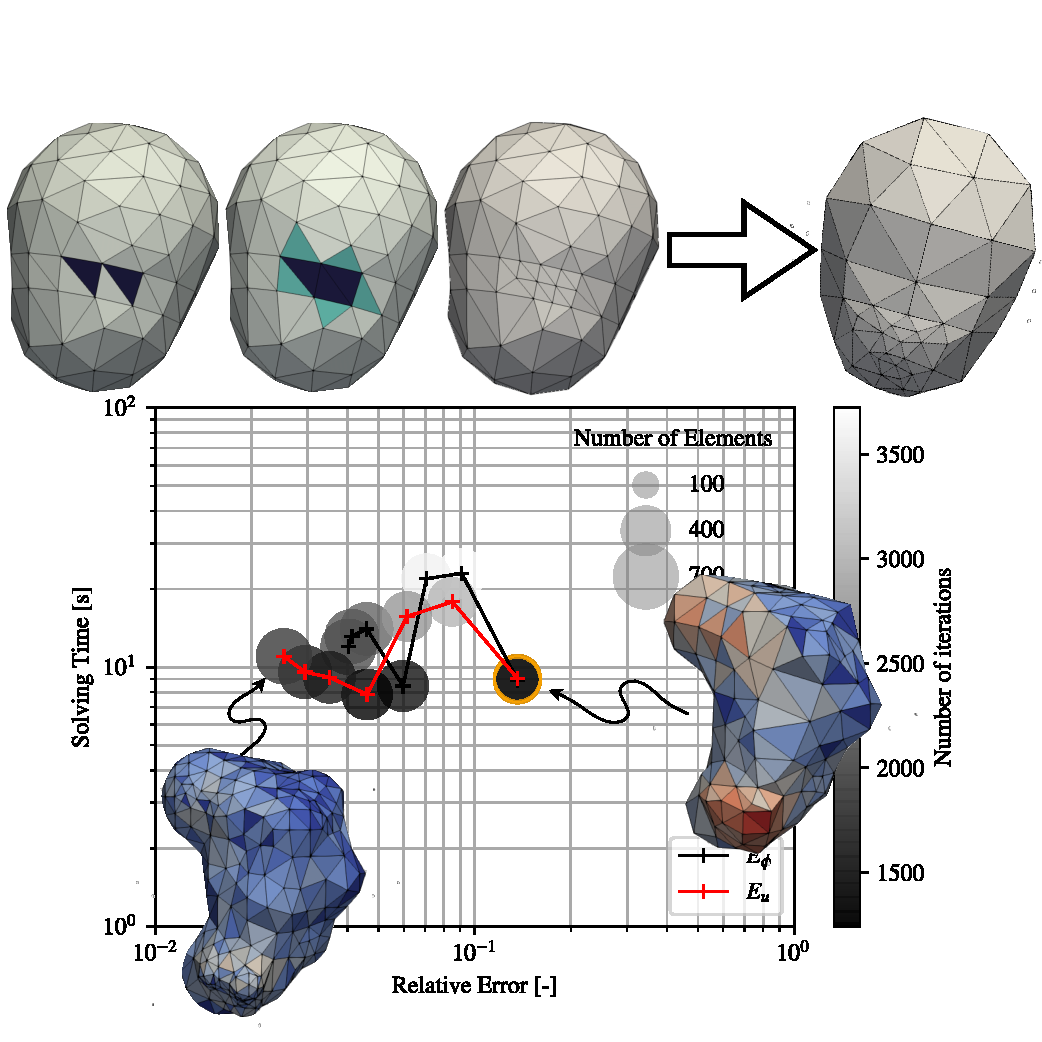
\includegraphics[width=50mm,height=50mm]{adaptive_mesh_fig.pdf} %Pick only one of the two styles by uncommenting the corresponding \includegraphics
%\includegraphics[width=110mm,height=20mm]{cc.eps}
\\
(75 words.) Images for the graphical Table of Contents should capture the essence of a paper, displaying a figure, plot, or scheme that is central to the theme of the manuscript. The text of the graphical Table of Contents is meant for the non-specialist and should ideally contain no obscure jargon or mathematical symbols / equations, but should attempt to convey the gist of the paper in everyday terms, while remaining consistent with accepted standards of scientific literature.
\end{minipage}
}}
\end{figure}

% makes references listed with 1., 2., etc.  
  \makeatletter
  \renewcommand\@biblabel[1]{#1.}
  \makeatother

\bibliographystyle{apsrev}

\renewcommand{\baselinestretch}{1.5}
\normalsize


\clearpage


\section*{\sffamily \Large INTRODUCTION} % Not needed for rapid communications

In biologically relevant settings, the structure and function of biomolecules is largely determined by the surrounding water with salt. 
To describe these systems accurately, we need to account for the solvent correctly, which has given rise to a wide range of models [cite water review]
Highly detailed models consider every water molecule and salt ion explicitly, however, there are approximated models that use continuum theory to represent this ionic solution, knwon as implicit-solvent models [SimonsonRoux, DescherchiRocchia].
In the case of electrostatics, the implicit-solvent model is mathematically characterized by the Poisson-Boltzmann equation (PBE) [Baker,Bardhan], which is widely used to compute solvation free energies and mean-field potentials.

The implicit-solvent model for electrostatics describes the dissolved molecule as a infinite medium with a low-dielectric solute-shaped cavity, which contains a charge distribution from the partial charges (usually a sum of Dirac deltas at the atom's locations).
The outer solvent region is represented with a high dielectric, and considers the presence of salt.
These two regions are interfaced by the molecular surface, which can be defined in various ways [cite], where the continuity of the electrostatic potential and electric displacement are enforced.

The PBE has been solved numerically with finite difference [cite], finite element [cite], boundary element [cite], and analytical [cite] methods.
In particular, the boundary element method (BEM) has proven to be very efficient for high accuracy calculations [GengKrasny2013,CooperBardhanBarba2014], mainly due to the precise description of the molecular surface and point charges. 
However, BEM is limited to constant material properties in each region, and the linear version of the PBE. 
Even though these limitations are acceptable in a wide range of applications, there are cases when BEM falls short, for example, if a variable permittivity is required inside the solute [cite], or the solute is highly charged such that the linear approximation breaks [cite?].

This article presents a methodology to overcome some of those limitations, through coupling boundary and finite elements (FEM-BEM).
This approach brings the best of both worlds: the flexibility of FEM and efficiency of BEM, all in an accurate description of the dissolved molecule.

% The opening sentence of the manuscript should summarize the reasons for the undertaking of the work and the main conclusions that can be drawn.

%((Place Introduction here))

%((Main text paragraphs should be 12 point font, double-spaced. Reviews are comprehensive survey of recent progress in a topic of broad interest in quantum chemistry, providing the readership with an appreciation of the importance of the work, a summary of recent developments, and a guide to the relevant literature. Perspective are short discussions of an important emerging topics in quantum chemistry, usually focused on no more than a few recently published papers, and including the authors' vision for the future of the topics, identifying important problems that should be addressed next. Perspective should be limited to 3000 words, 4 display items (figures and/or tables), and 30 references.))

%((Full Papers are comprehensive reports of important recent advances in the development of basic theory, quantum mechanical computational methodologies and their relevant applications that provide significant insight to problems of broad interest in chemistry, physics, biology, and materials science. The opening sentence of the manuscript should summarize the reasons for the undertaking of the work and the main conclusions that can be drawn. The main text should be contain sections with brief subheadings, a summary of the major conclusions of the paper, and a Method section containing sufficient detail to reproduce the work. Main text paragraphs should be 12 point font, double-spaced.))

%((Rapid communications should be limited to 1500 words, 3 display items (figure and/or tables), 20 references. Main text paragraphs should be 12 point font, double-spaced. There are NO headings in the main text.))

\section*{\sffamily \Large METHODOLOGY}
\subsection*{\sffamily \large The implicit solvent model}

The implicit solvent model can be described mathematically as a coupled system of partial differential equations, where the Poisson-Boltzmann governs in the solvent region ($\Omega_X$ in Figure XX), and the Poisson equation in the solute region ($\Omega_Y$ in Figure XX). These regions are interfaced by the molecular surface ($\Gamma$), where the potential ($\phi$) and electric displacement ($\epsilon\partial\phi/\partial\mathbf{n}$) are continuous. 
%
\begin{align}\label{eq:pbe}
\nabla^2\phi_1(\mathbf{x}) &= \frac{1}{\epsilon}\sum_{k=1}^{N_q} q_k\delta(\mathbf{x},\mathbf{x}_k) \quad  \mathbf{x} \in \Omega_1\nonumber\\
\left(\nabla^2 - \kappa^2\right)\phi_2 &= 0 \quad\mathbf{x}\in\Omega_2\nonumber\\
\phi_1 = \phi_2 &\quad \epsilon_1\frac{\partial\phi_1}{\partial\mathbf{n}} = \epsilon_2\frac{\partial\phi_2}{\partial\mathbf{n}} \quad \mathbf{x}\in \Gamma. 
\end{align}
%
where $\epsilon_1$ and $\epsilon_2$ are the dielectric constants in the solute and solvent, respectively, $\kappa$ is the inverse of the Debye length, related with the salt concentration, and $q_k$ are the values of the partial charges, located at $\mathbf{x}_k$.

The electrostatic potential in $\Omega_1$ can be further decomposed into singular and regular components as $\phi_1 = \phi_c + \phi_R$, where $\phi_c$ is the solution to
%
\begin{align}\label{eq:phic}
\nabla^2\phi_c(\mathbf{x}) &= \frac{1}{\epsilon_1}\sum_{k=1}^{N_q}q_k\delta(\mathbf{x},\mathbf{x}_k) \quad \mathbf{x}\in\Omega_1\cup\Omega_2\nonumber\\
\phi_c(\mathbf{x})&=0 \quad \text{ as } |\mathbf{x}|\to\infty
\end{align}

Physically, $\phi_c$ can be interpreted as the Coulomb-type potential from the point charges, whereas $\phi_R$, also known as reaction potential, is originated by the polarization of the solvent. 
Usually, $\epsilon_1$ is considered a constant value, yielding an analytical expression for $\phi_c$. 
However, the molecule permittivity may vary in space, in which case we need to solve Equation \eqref{eq:phic} numerically.

There are regularized versions of Equation \eqref{eq:pbe} [HolstETal2008,GengZhao2020] which are widely used to numerically solve the Poisson-Boltzmann equation with finite element or finite difference methods.
However, here we use the standard formulation in Equation \eqref{eq:pbe}, as it offers more flexibility when dealing with, for example, variable permitivitties.

A common quantity of interest in implicit solvent models is the solvation free energy, which the change in Gibbs free energy as the molecule moves from vacuum into the solvent. Considering the charge distribution $\rho$ consists of point charges, this can be calculated as
%
\begin{equation}\label{eq:dG}
\Delta G_{solv} = \frac{1}{2}\int_{\Omega_1} \rho(\mathbf{x})\phi_{r}(\mathbf{x}) = \frac{1}{2}\sum_{k=1}^{N_q} q_k\phi_r(\mathbf{x_k})
\end{equation}

\subsection*{\sffamily \large Numerical solution of the Poisson-Boltzmann equation}

\subsection*{\sffamily \large BEM-BEM coupling}

\subsection*{\sffamily \large FEM-BEM coupling}




\begin{itemize}
    \item Implicit solvent model and Poisson-Boltzmann 
    \item Regularized PB (3-term splitting)
    \item Description with constant and variable permittivity 
    \item Standard BEM-BEM and FEM-BEM coupling approach
    \item Hybrid FEM-BEM coupling
\end{itemize}


%((Place Computational Methods here. Not needed for review articles))

%((Computational results should be prepared following the IUPAC guidelines (See Journal of Computational Chemistry, 20: 1587-1590 and 20:1591-1592). In particular, it is required that the level of theory employed is appropriate to the problem at hand, and that the sufficient details about methodology are provided to allow the work to be reproduced.)

%((In full papers, this section appears immediately after the introduction. In Rapid Communications, this section appears just before the Acknowledgments.))

\section*{\sffamily \Large RESULTS}
\section*{\sffamily \Large Results with constant permitivitty}

\subsection*{\sffamily \large Convergence of a spherical cavity}
\begin{itemize}
    \item Show convergence to analytical solution for
    \begin{itemize}
        \item BEM-BEM
\begin{figure}[!htb]
\minipage{0.32\textwidth}
  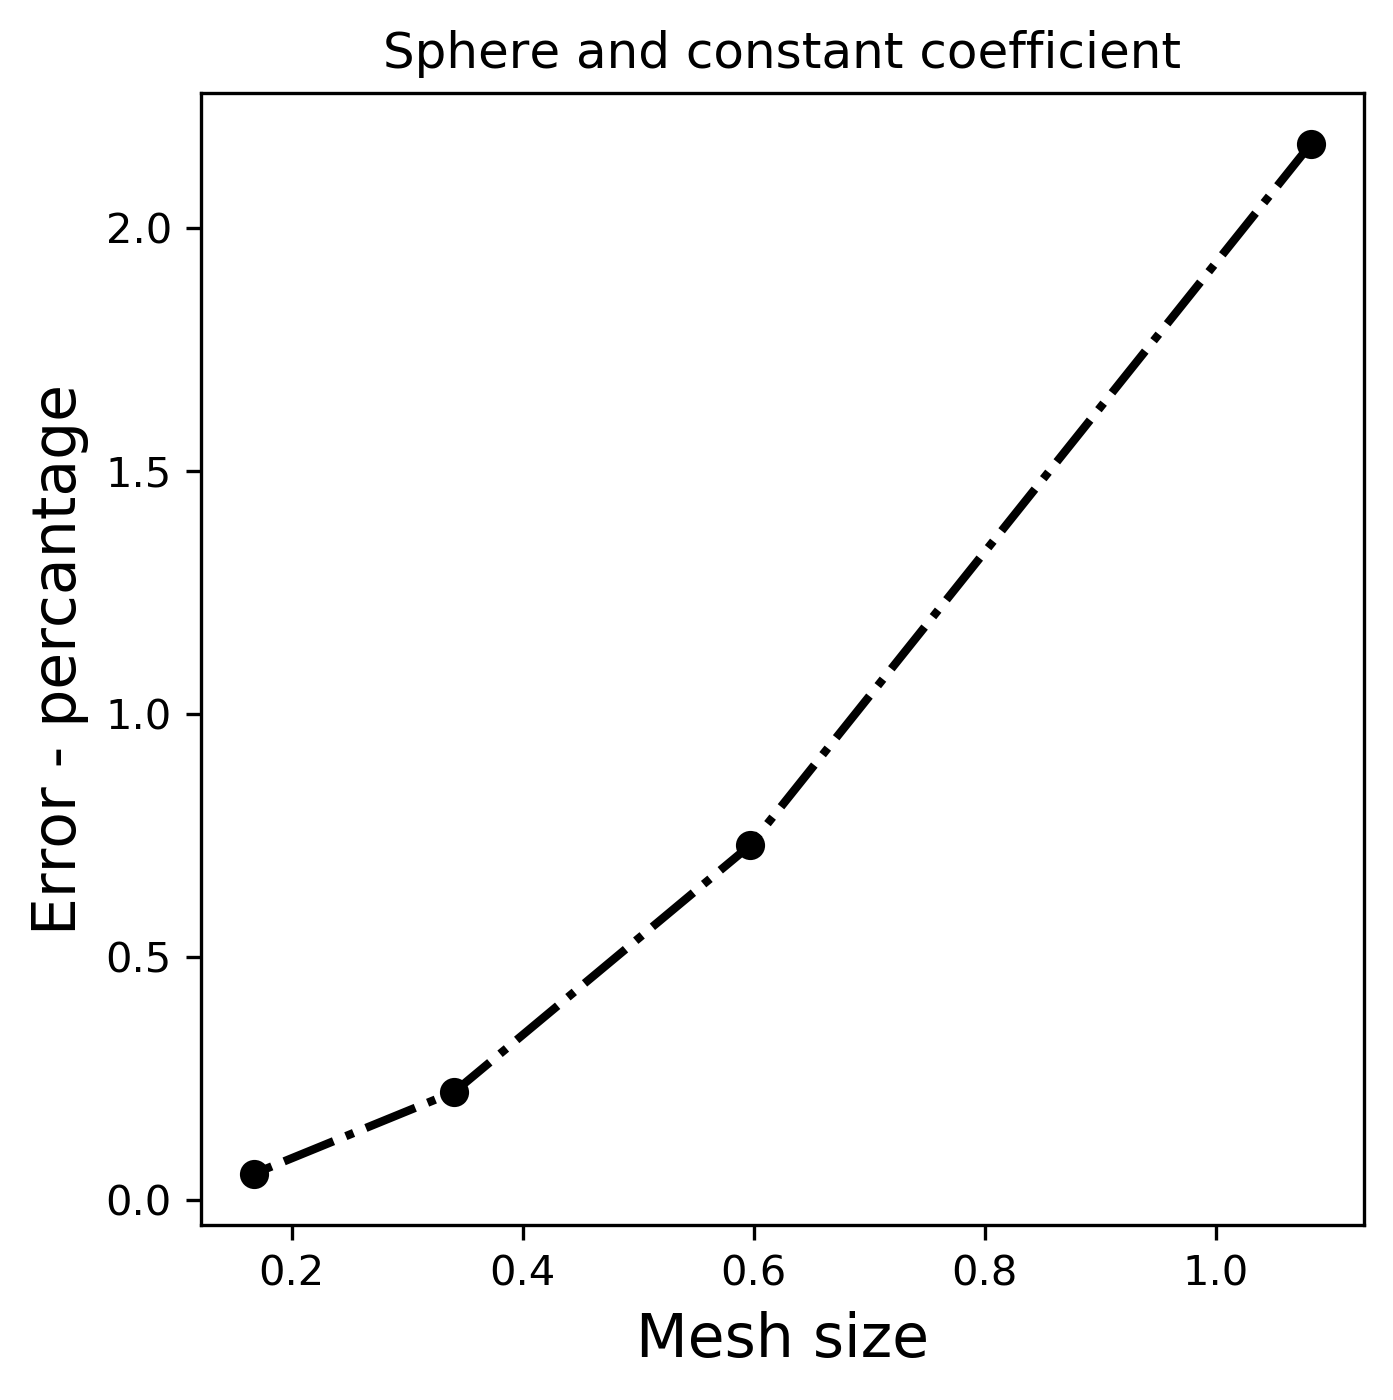
\includegraphics[width=\linewidth]{BEM_BEM_Sphere_const_coeff_error.png}
  \caption{Error}
\endminipage\hfill
\minipage{0.32\textwidth}
  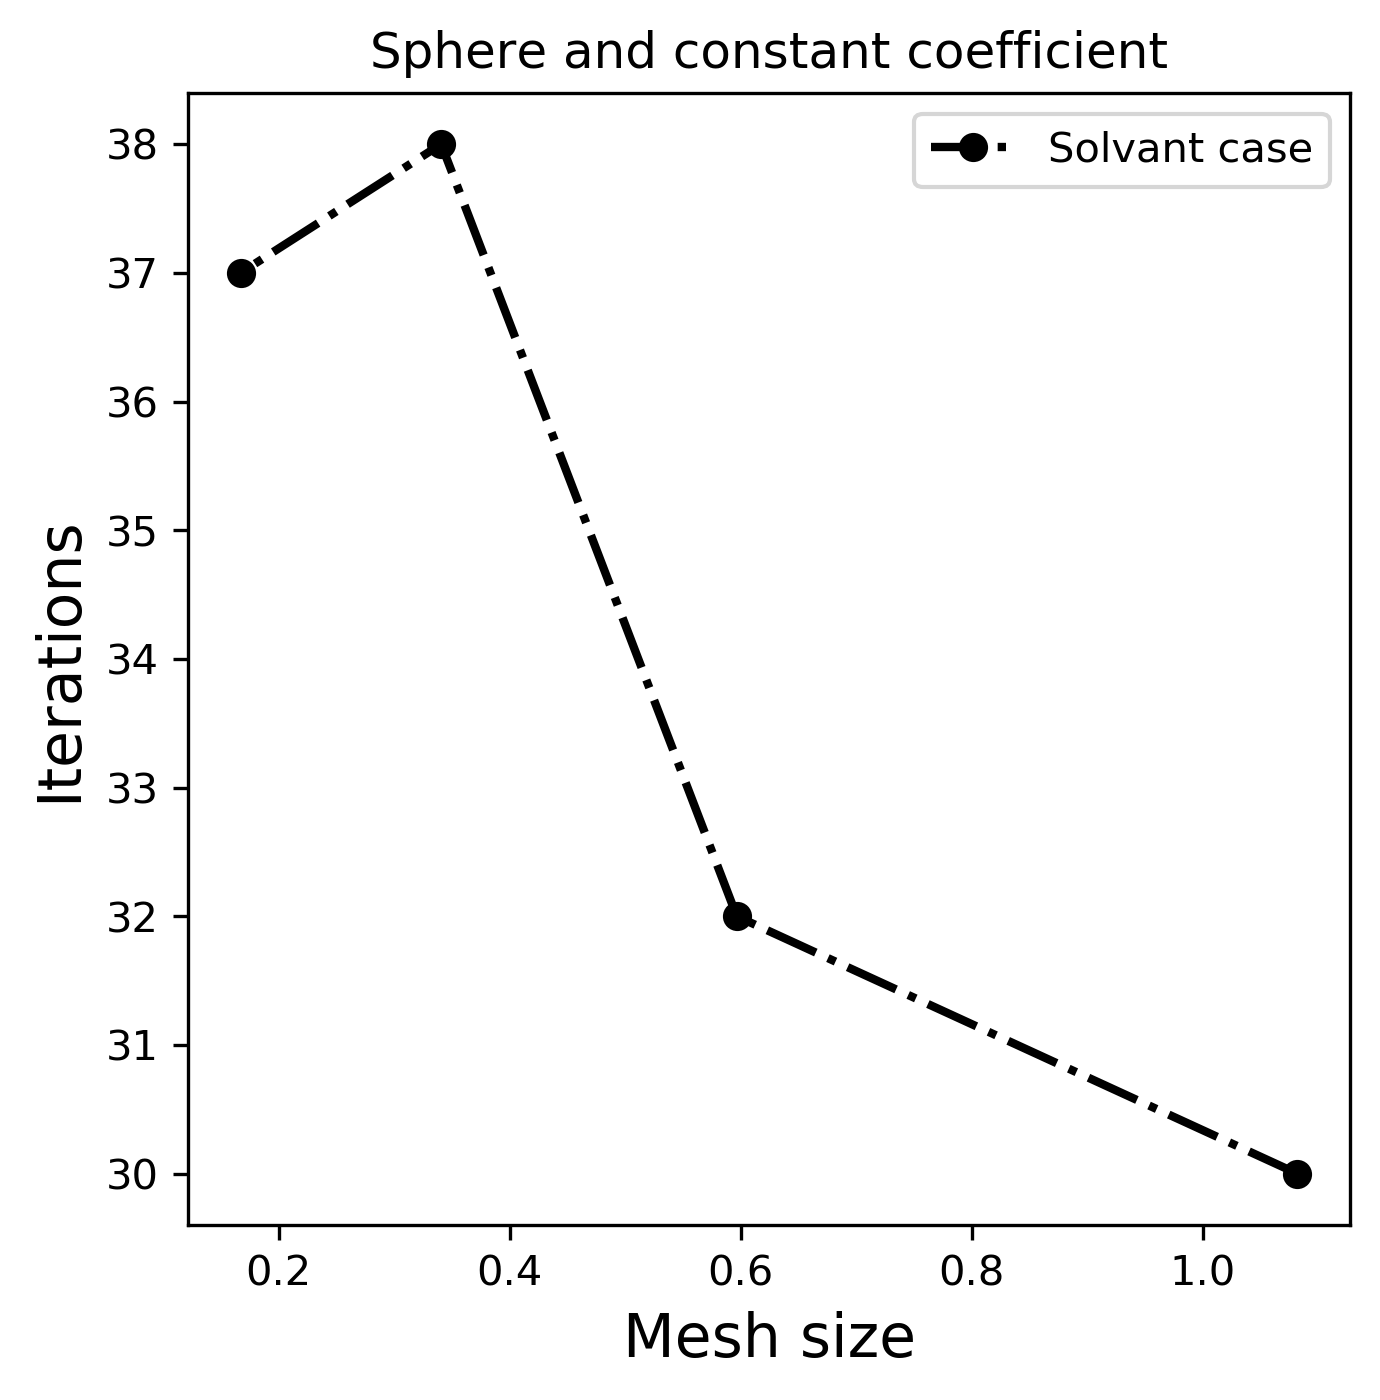
\includegraphics[width=\linewidth]{BEM_BEM_Sphere_const_coeff_iter.png}
  \caption{Iterations}
\endminipage\hfill
\minipage{0.32\textwidth}%
  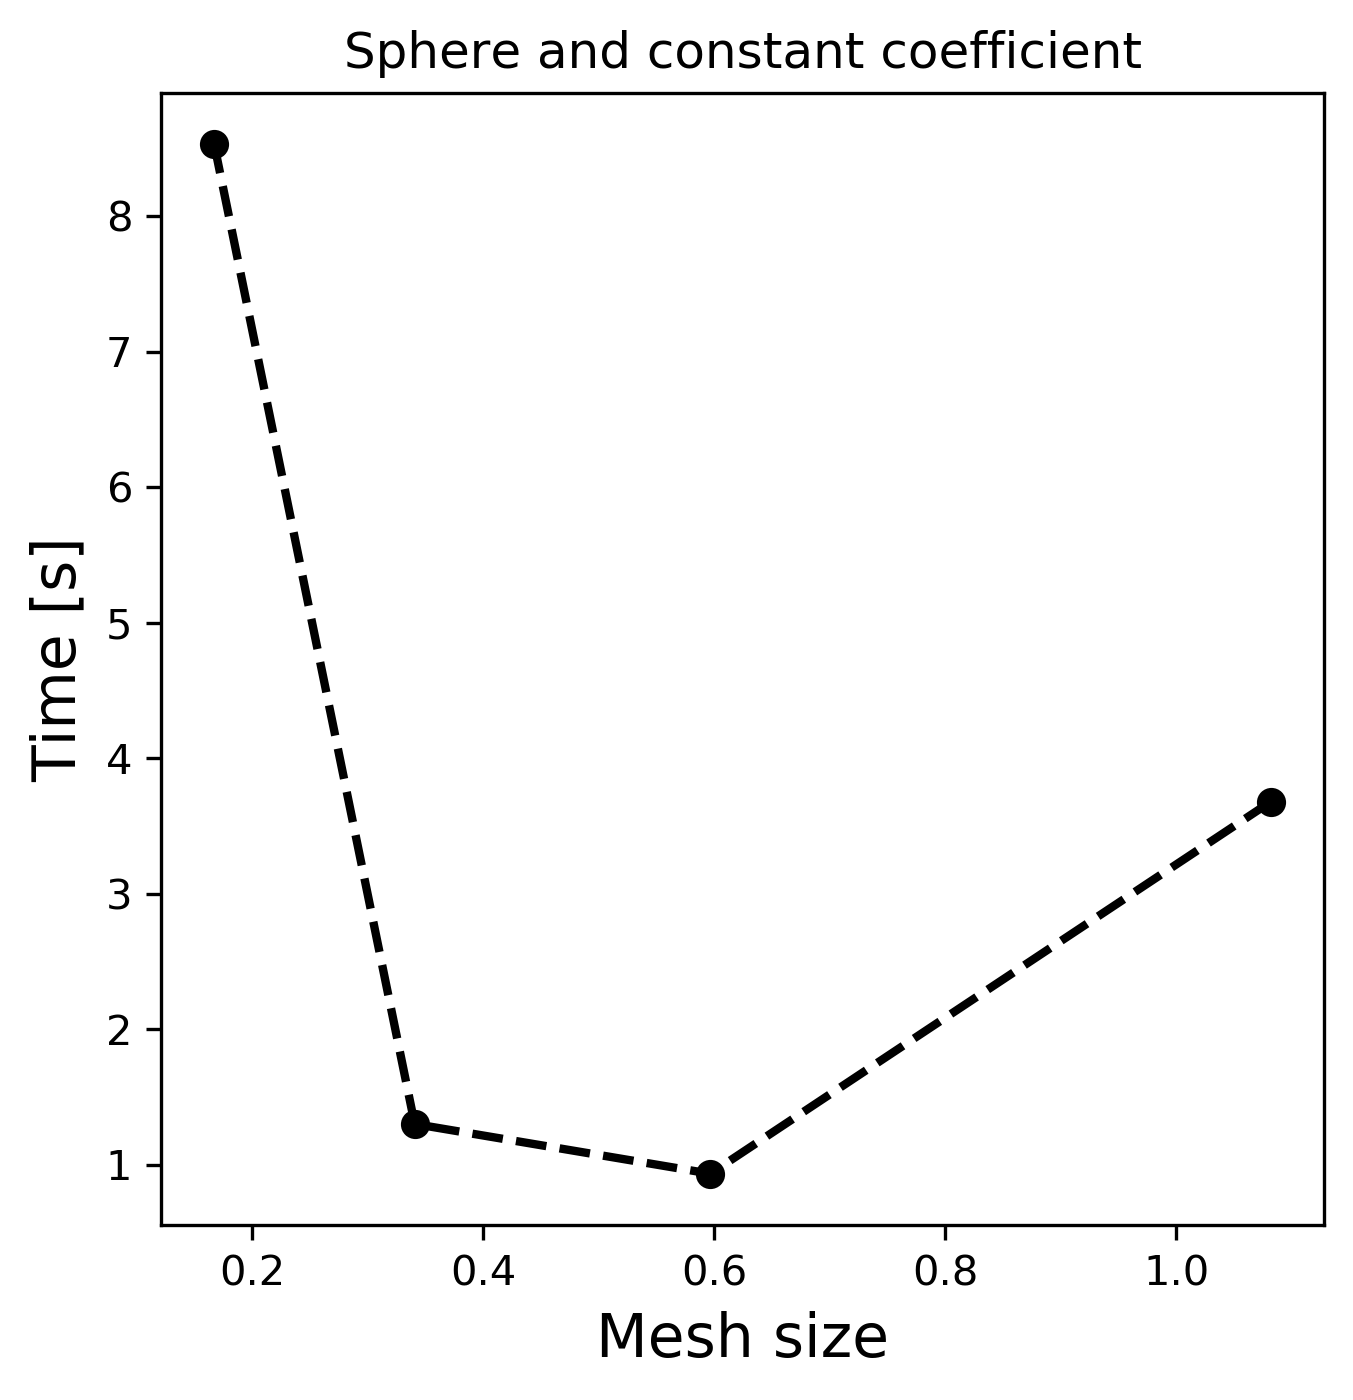
\includegraphics[width=\linewidth]{BEM_BEM_Sphere_const_coeff_time.png}
  \caption{Computational time}
\endminipage
\end{figure}
        \item Standard FEM-BEM
\begin{figure}[!htb]
\minipage{0.32\textwidth}
  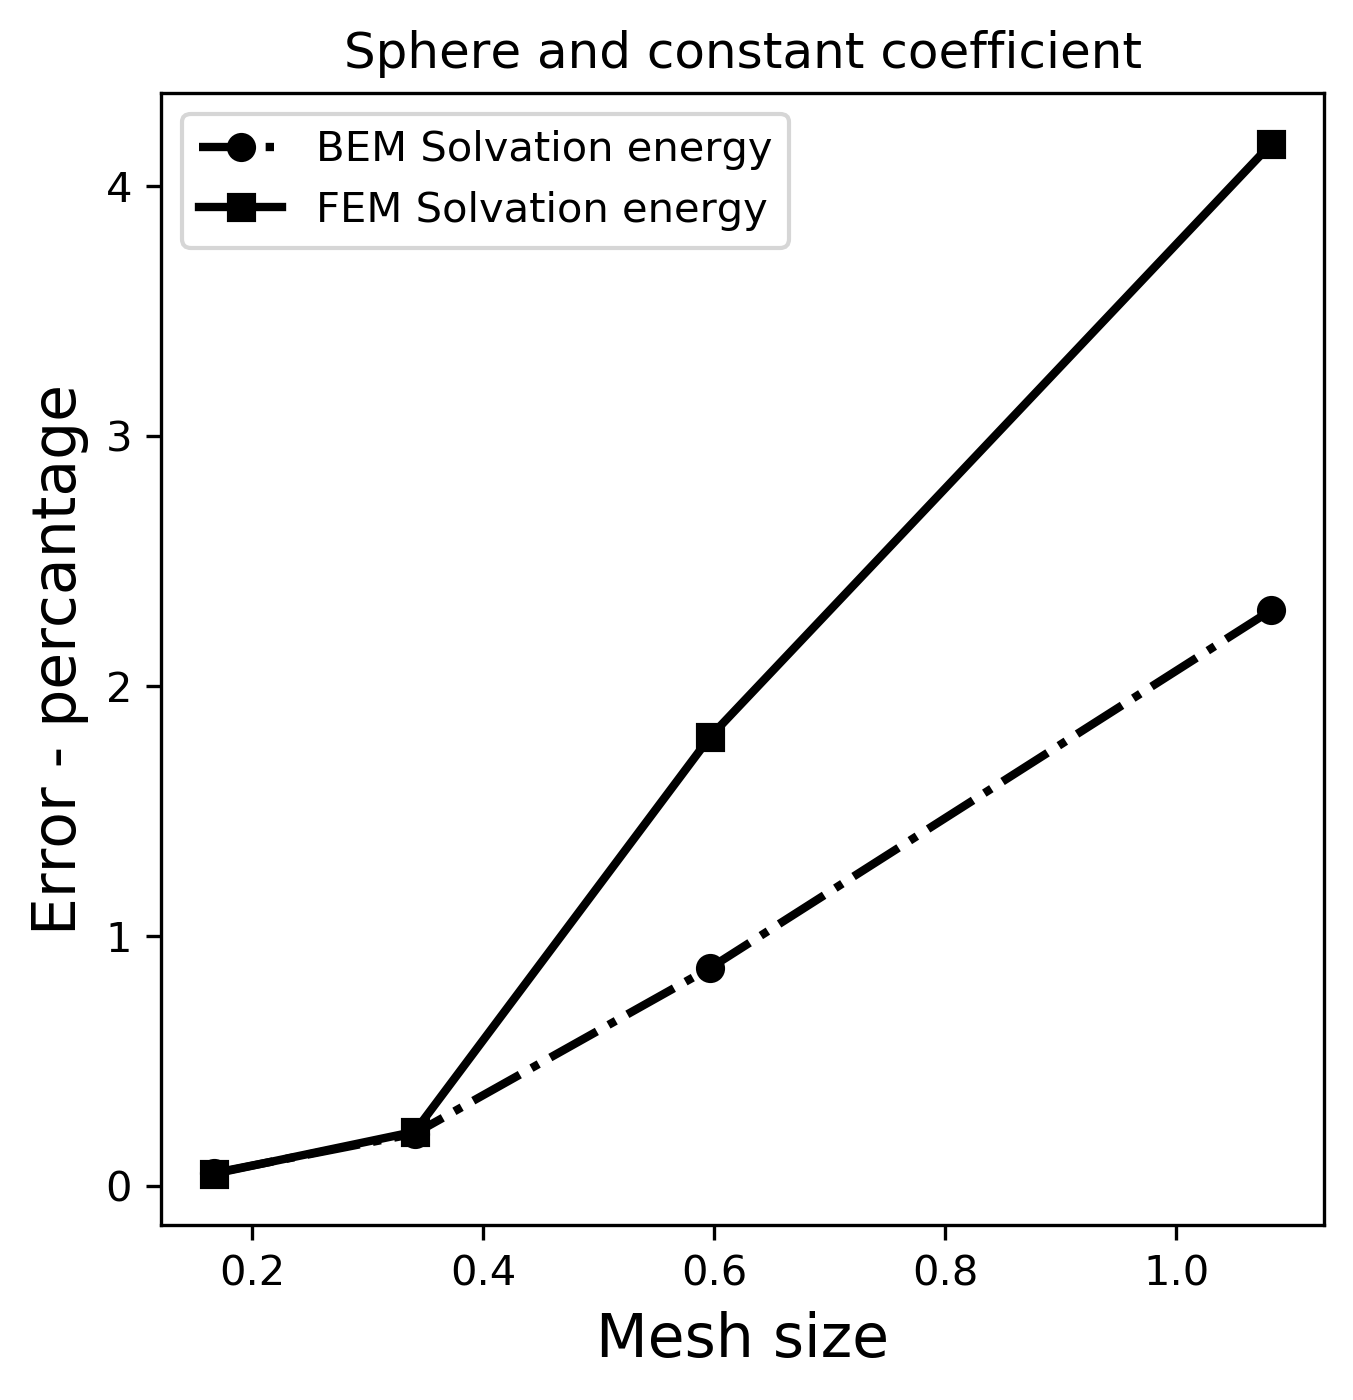
\includegraphics[width=\linewidth]{FEM_BEM_Sphere_const_coeff_error.png}
  \caption{Error}
\endminipage\hfill
\minipage{0.32\textwidth}
  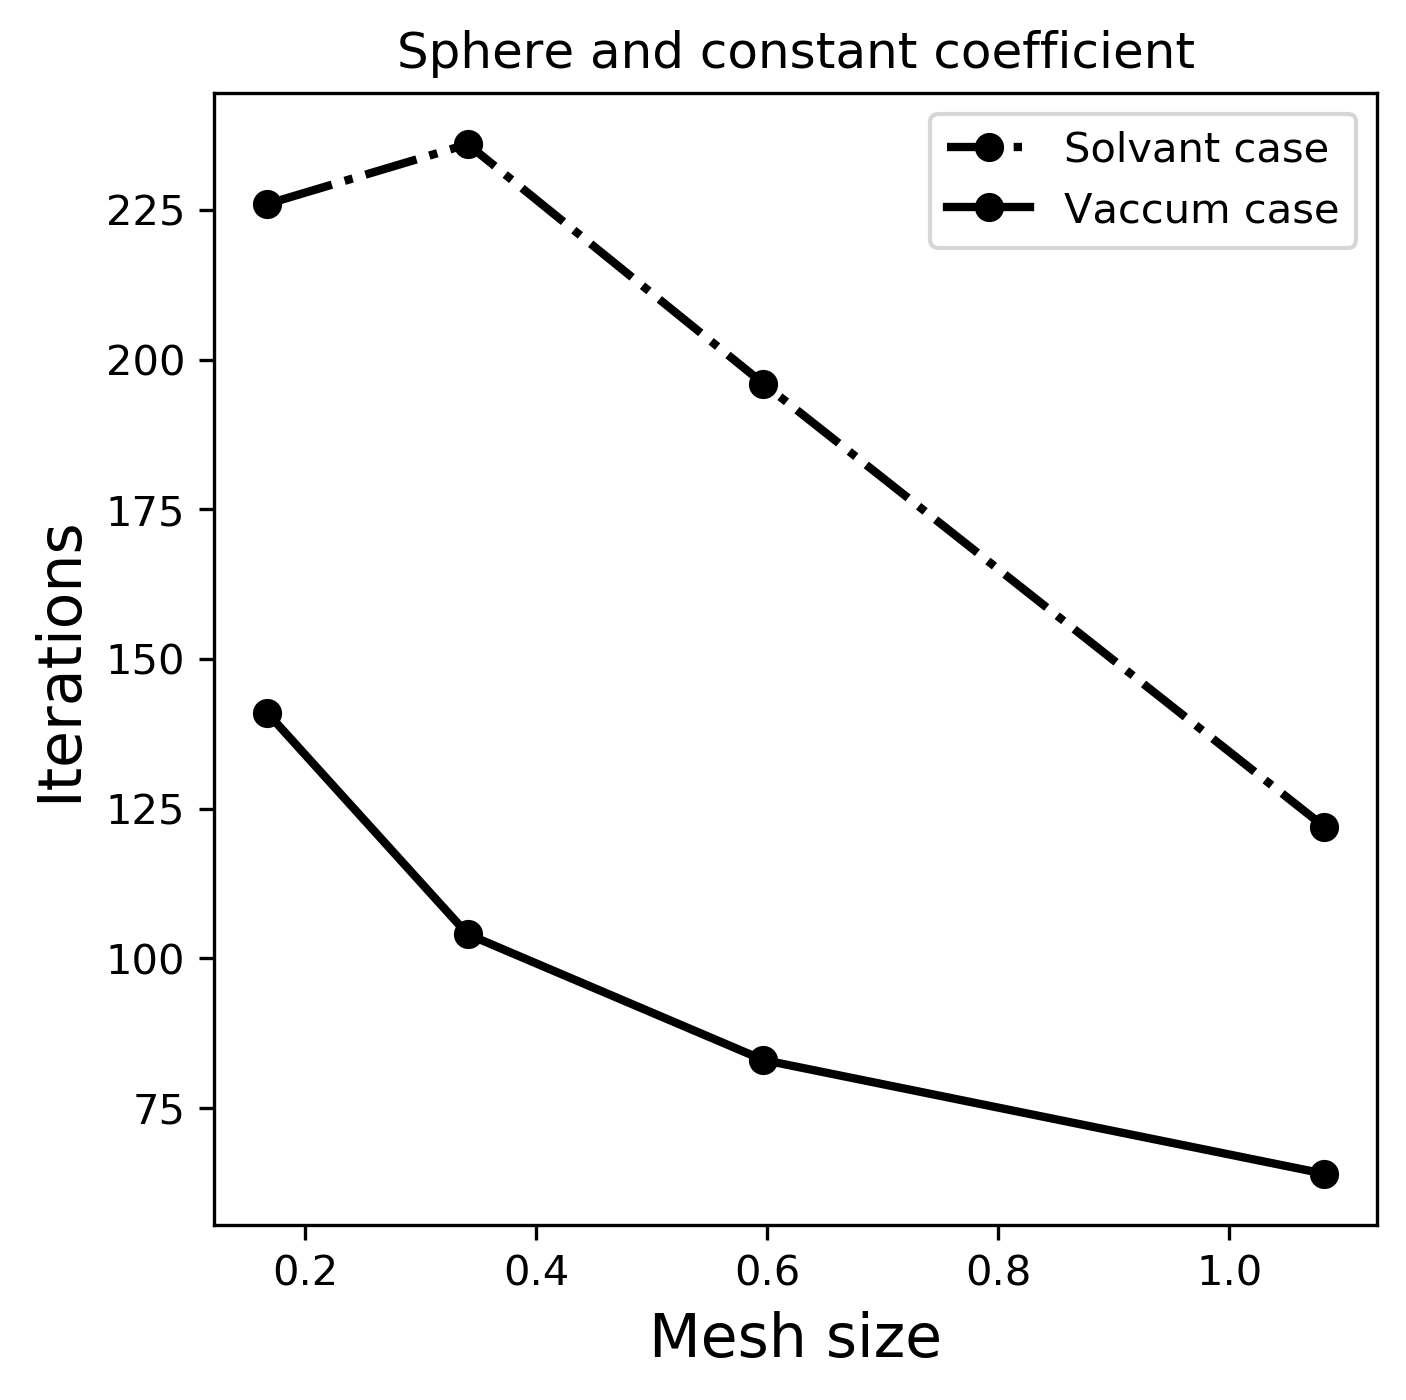
\includegraphics[width=\linewidth]{FEM_BEM_Sphere_const_coeff_iter.png}
  \caption{Iterations}
\endminipage\hfill
\minipage{0.32\textwidth}%
  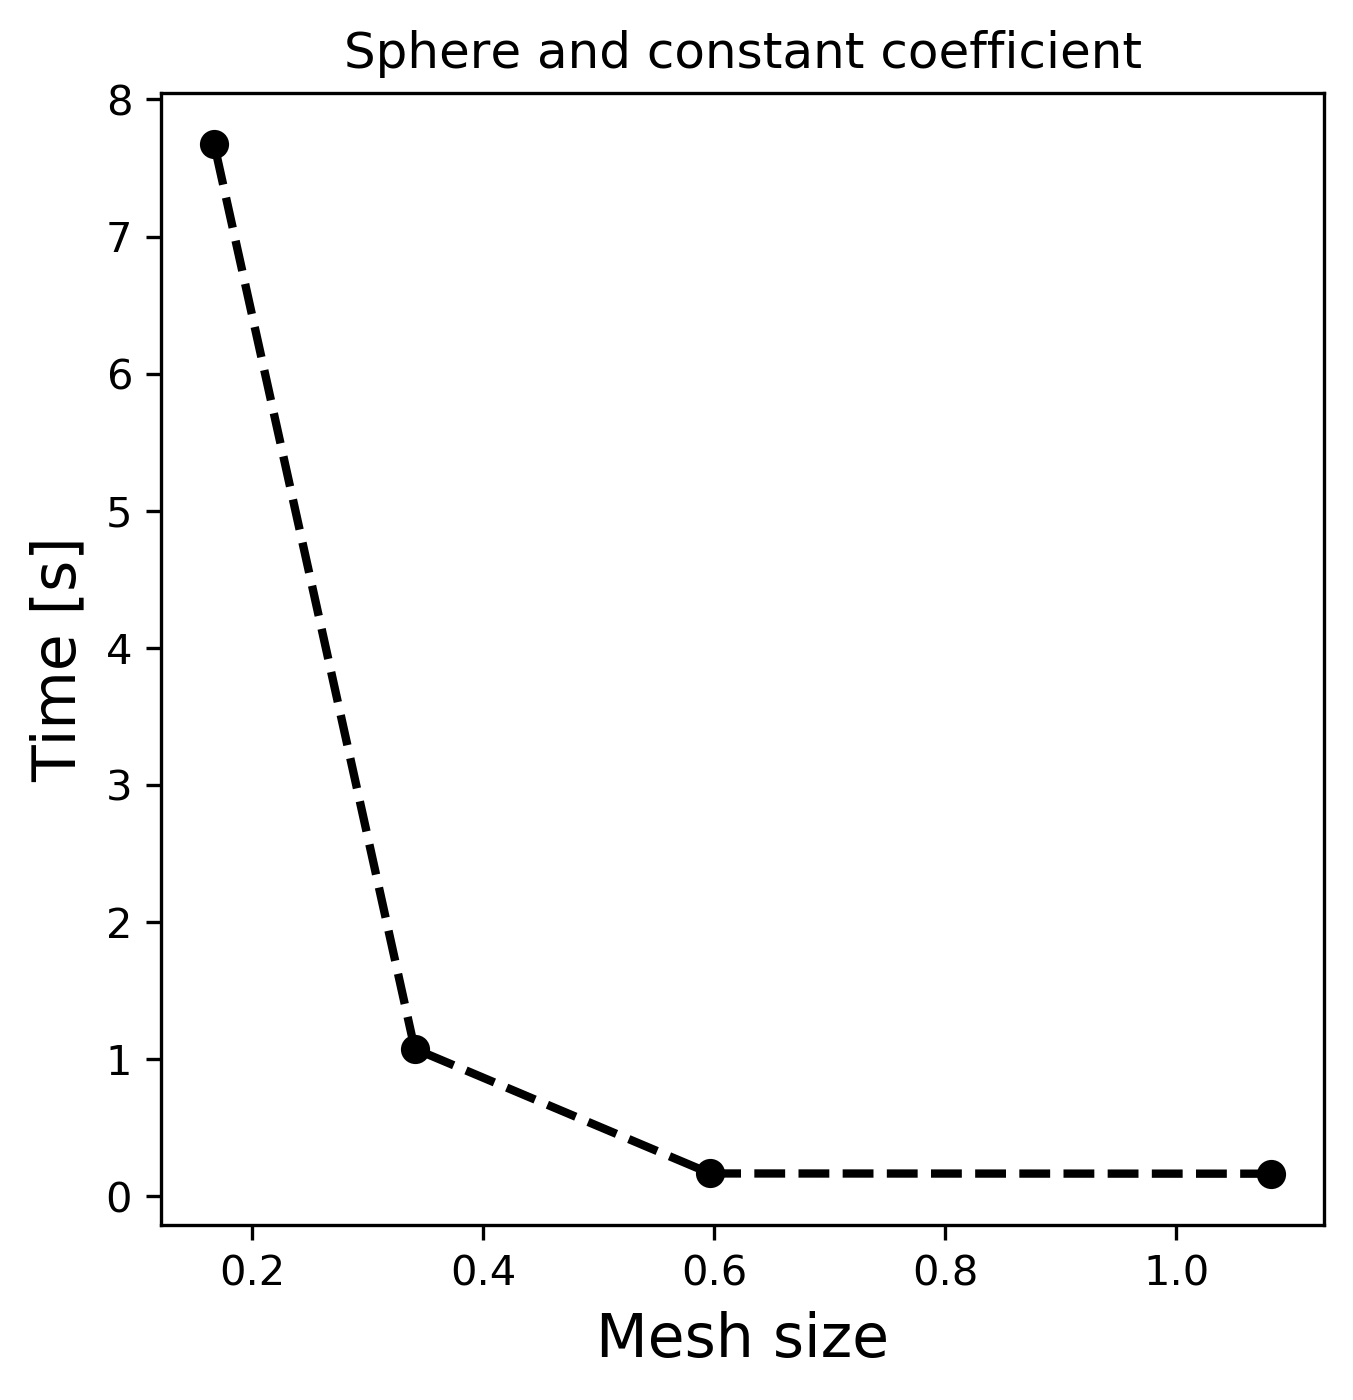
\includegraphics[width=\linewidth]{FEM_BEM_Sphere_const_coeff_time.png}
  \caption{Computational time}
\endminipage
\end{figure}
        \item Hybrid FEM-BEM
\begin{figure}[!htb]
\minipage{0.32\textwidth}
  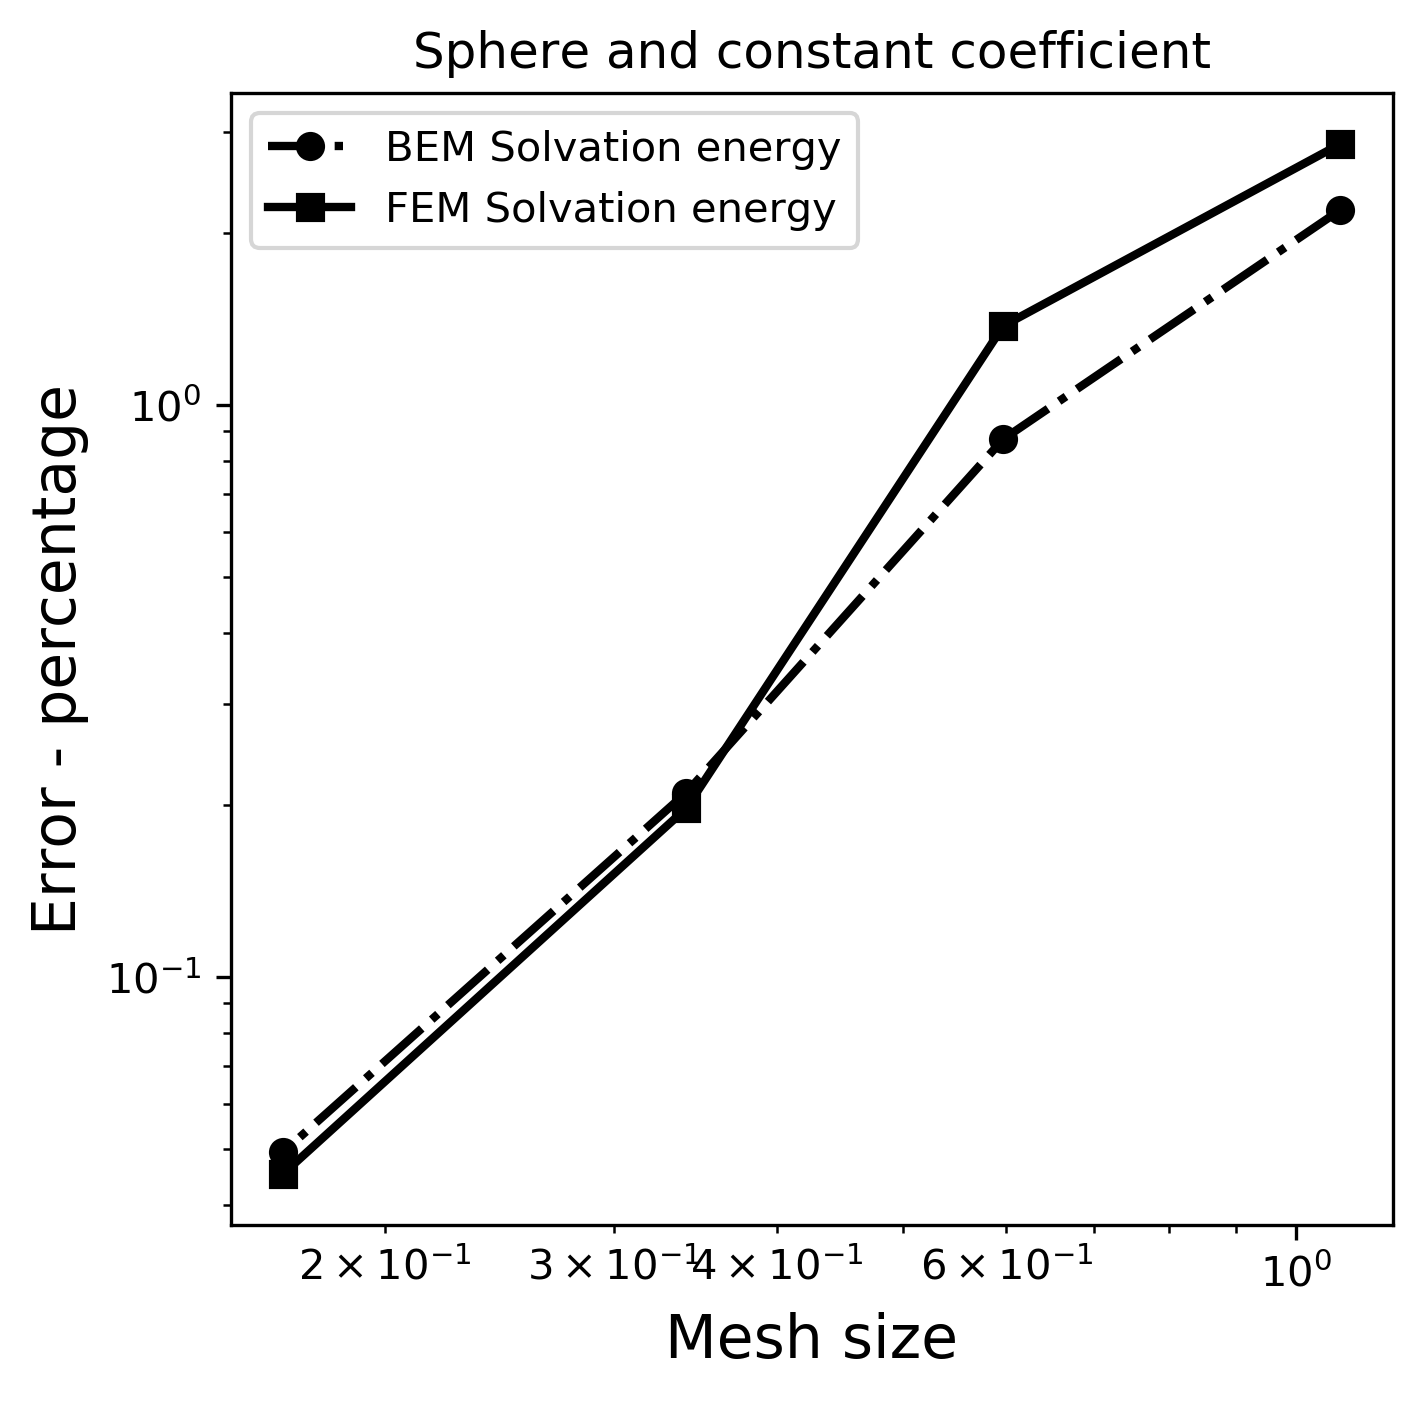
\includegraphics[width=\linewidth]{Hybrid_FEM_BEM_Sphere_const_coeff_error.png}
  \caption{Error}
\endminipage\hfill
\minipage{0.32\textwidth}
  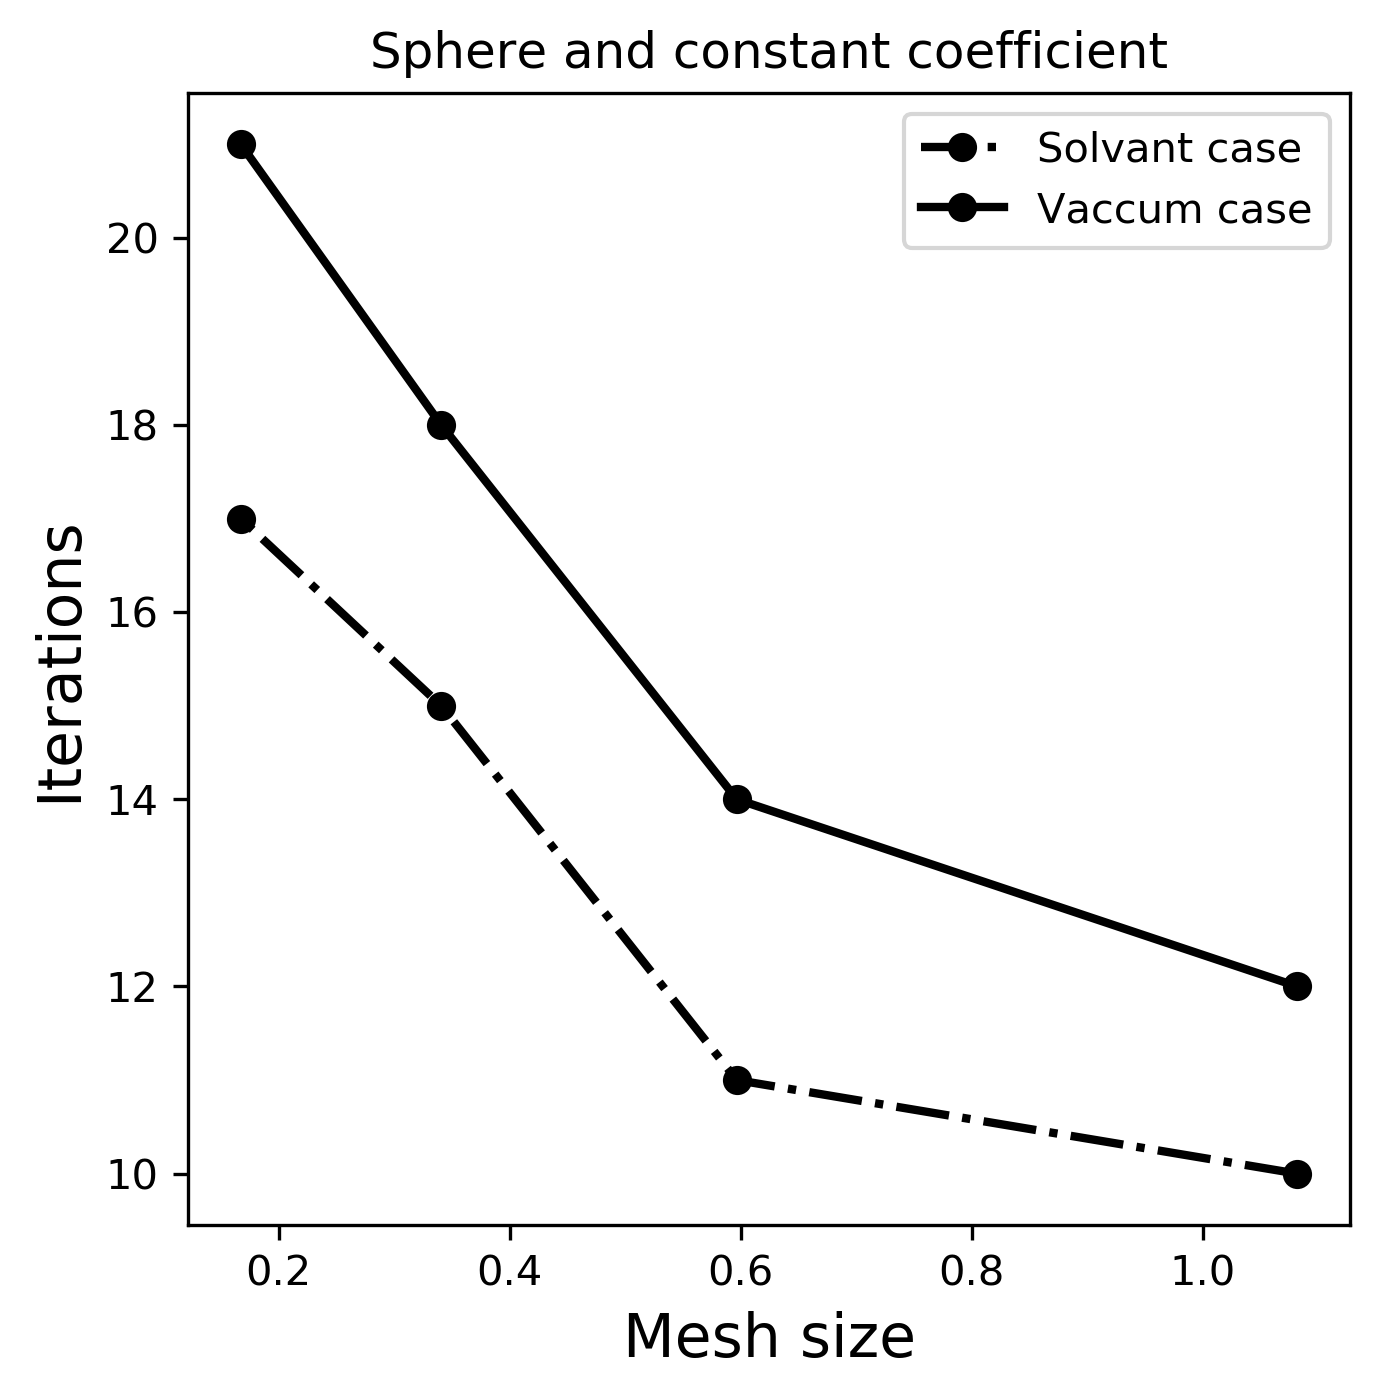
\includegraphics[width=\linewidth]{Hybrid_FEM_BEM_Sphere_const_coeff_iter.png}
  \caption{Iterations}
\endminipage\hfill
\minipage{0.32\textwidth}%
  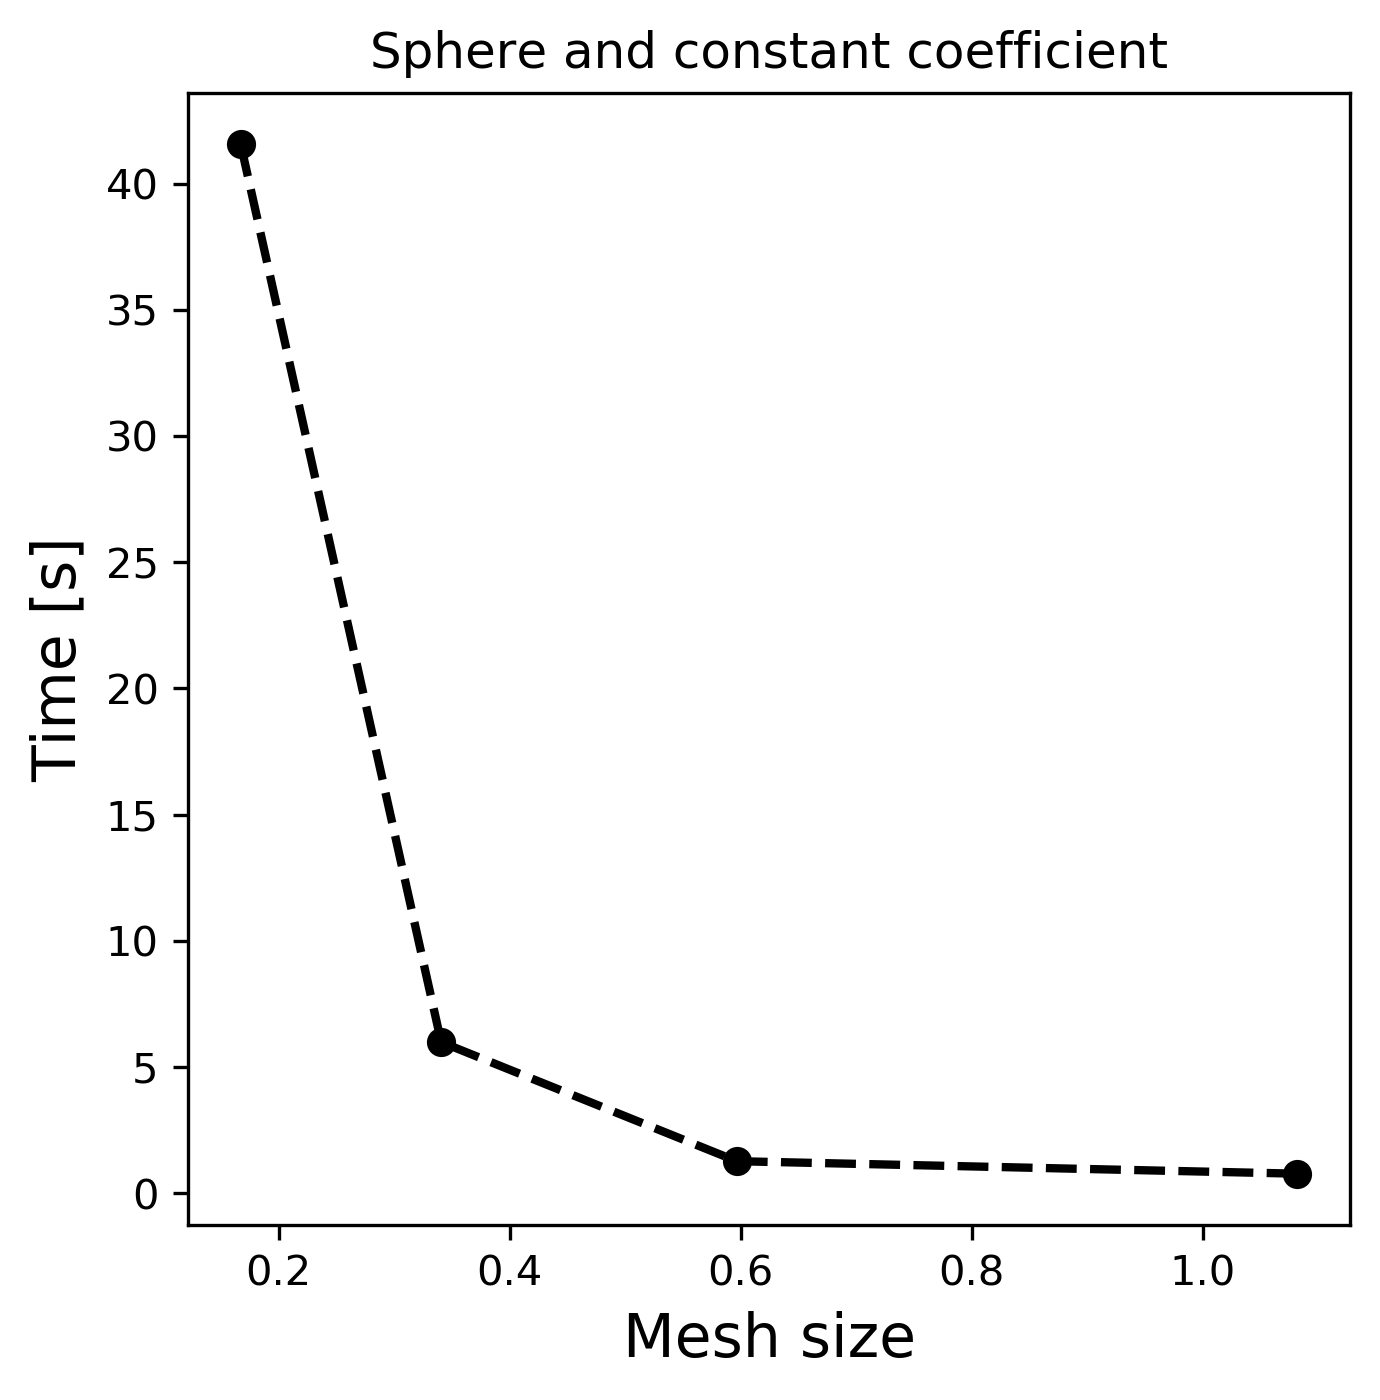
\includegraphics[width=\linewidth]{Hybrid_FEM_BEM_Sphere_const_coeff_time.png}
  \caption{Computational time}
\endminipage
\end{figure}
    \end{itemize}
\end{itemize}

\subsection*{\sffamily \large Performance for a molecular geometry}
\begin{itemize}
    \item Use arginine or a small protein (1PGB?)
    \begin{itemize}
        \item BEM-BEM
\begin{figure}[!htb]
\minipage{0.45\textwidth}
  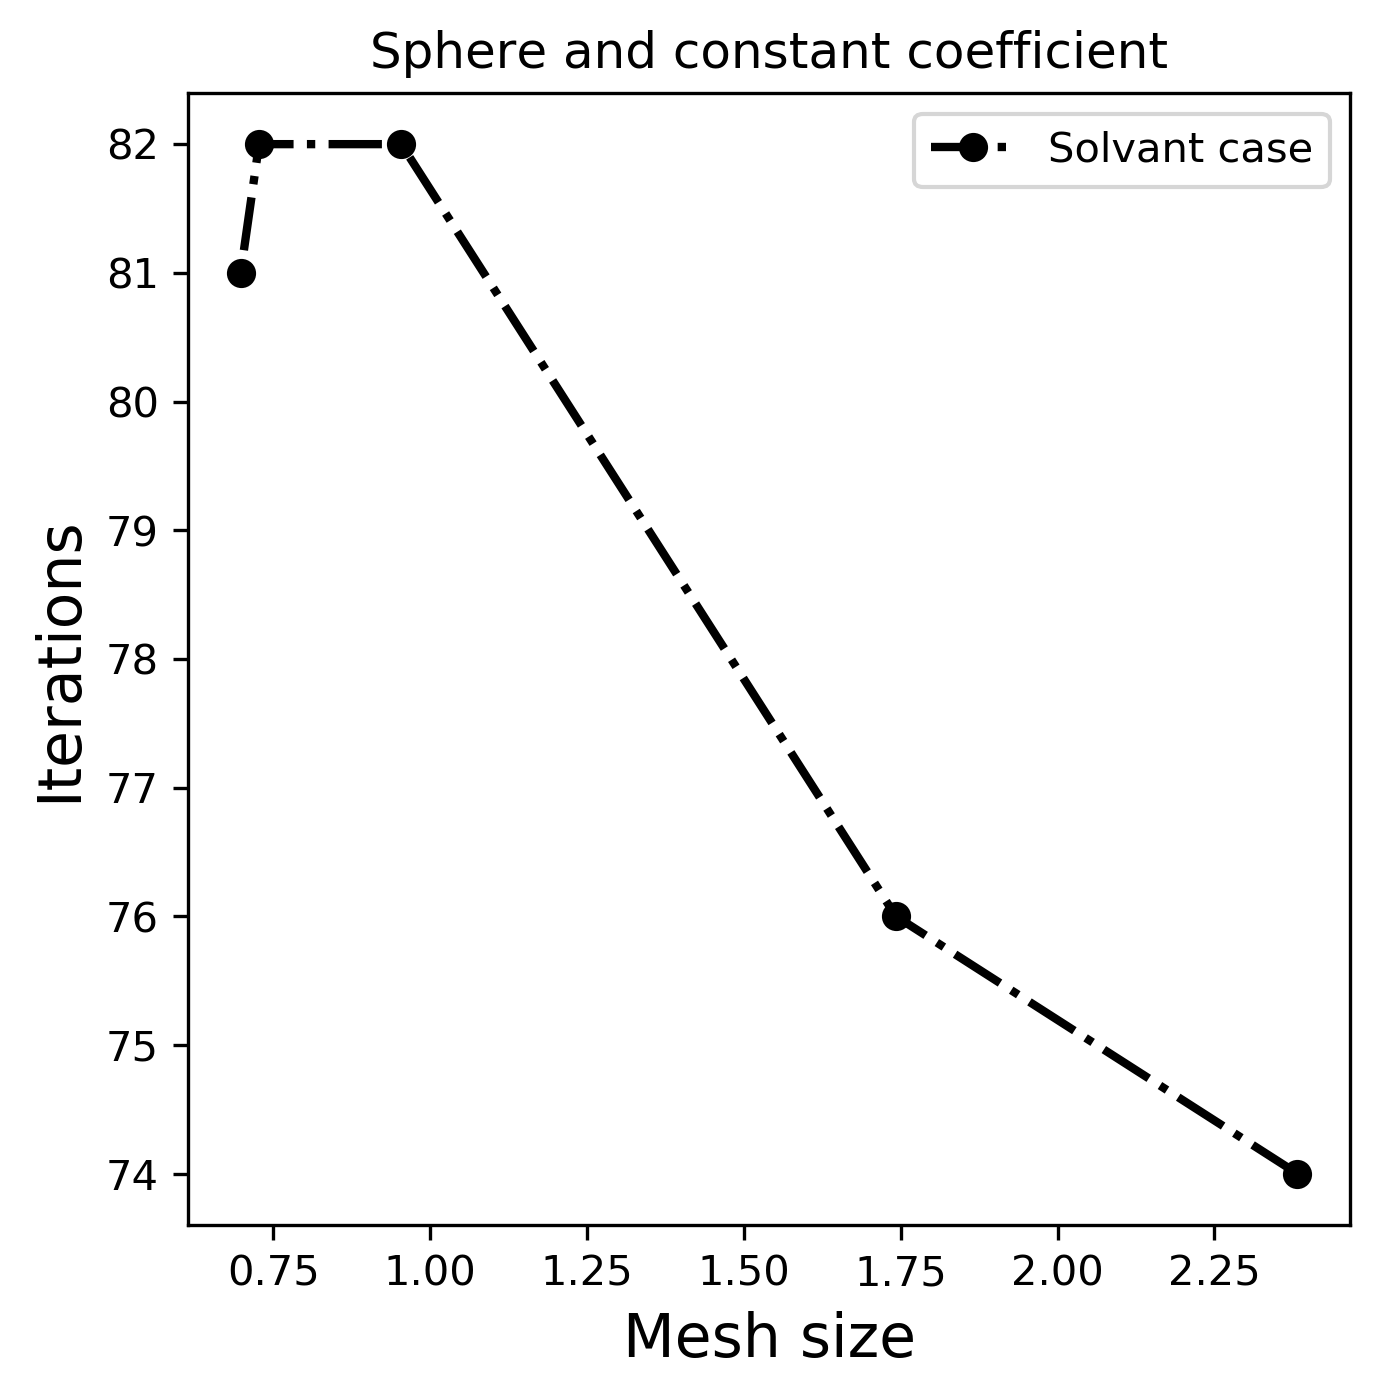
\includegraphics[width=\linewidth]{BEM_BEM_Arginine_const_coeff_iter.png}
  \caption{Iterations}
\endminipage\hfill
\minipage{0.45\textwidth}%
  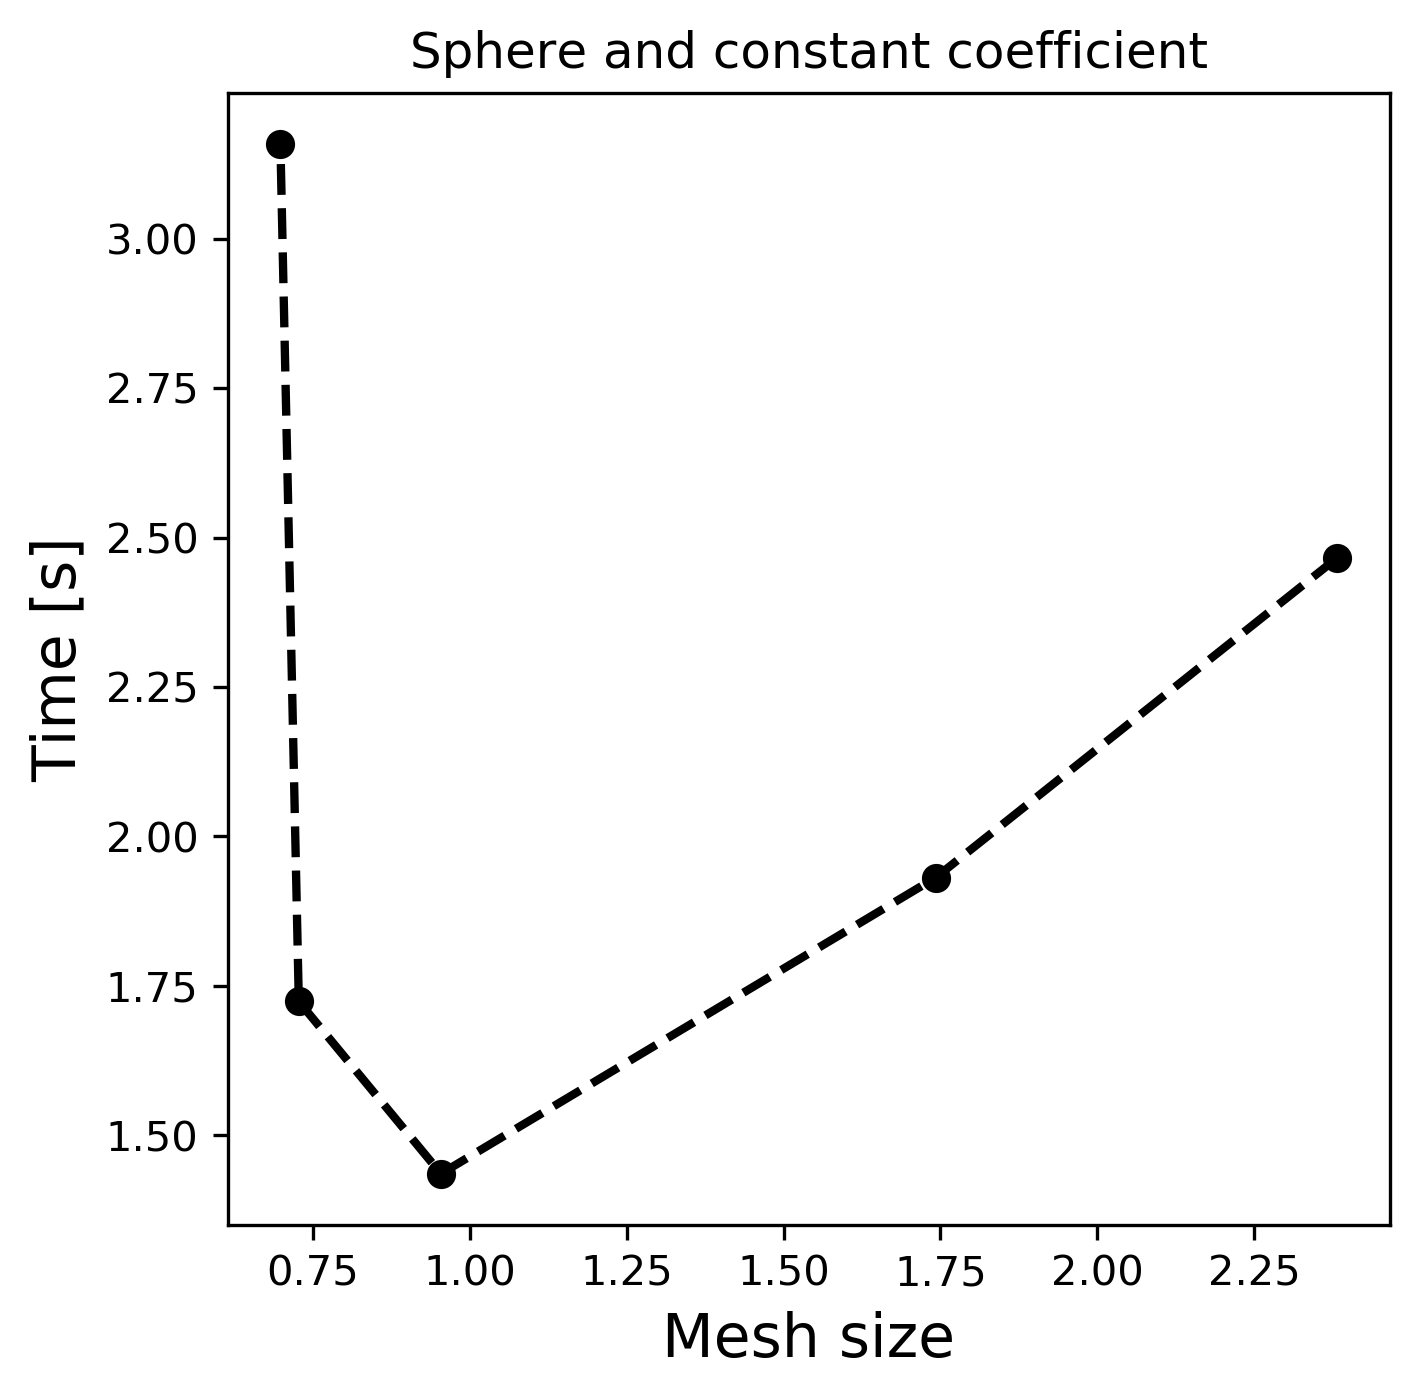
\includegraphics[width=\linewidth]{BEM_BEM_Arginine_const_coeff_time.png}
  \caption{Computational time}
\endminipage
\end{figure}
        \item Standard FEM-BEM
\begin{figure}[!htb]
\minipage{0.45\textwidth}
  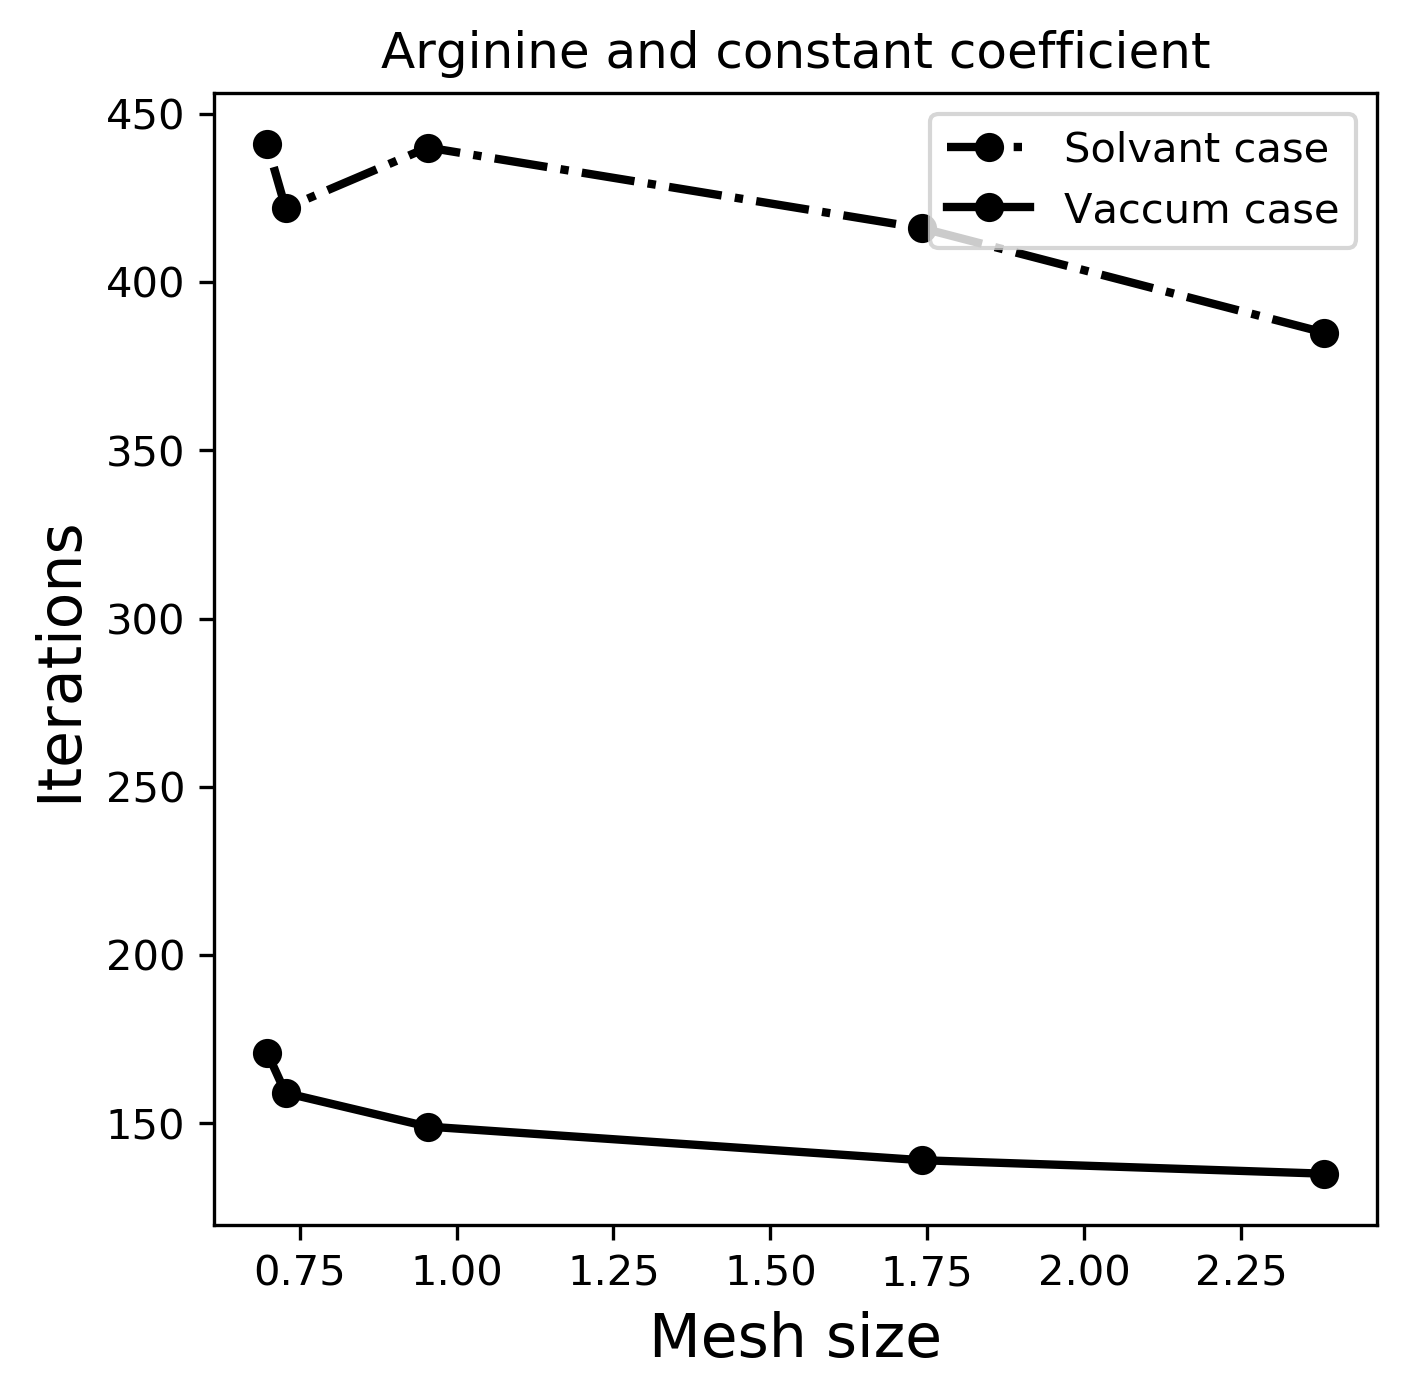
\includegraphics[width=\linewidth]{FEM_BEM_Arginine_const_coeff_iter.png}
  \caption{Iterations}
\endminipage\hfill
\minipage{0.45\textwidth}%
  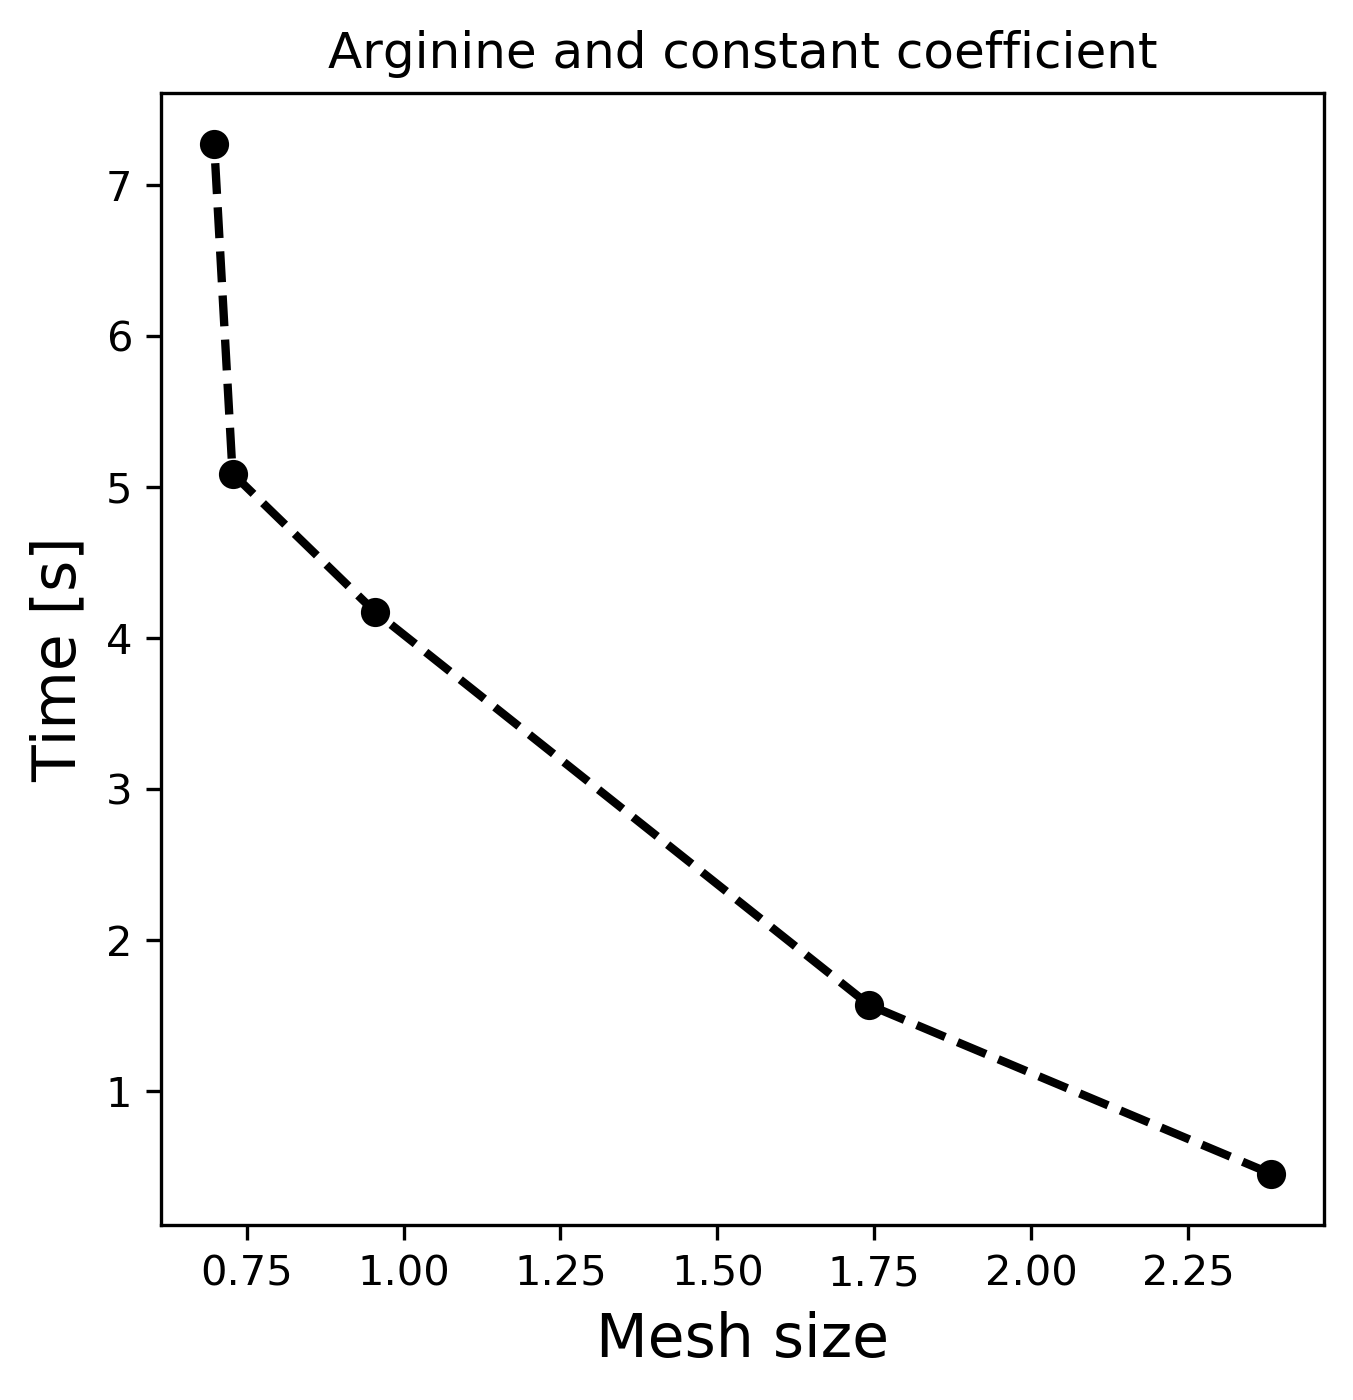
\includegraphics[width=\linewidth]{FEM_BEM_Arginine_const_coeff_time.png}
  \caption{Computational time}
\endminipage
\end{figure}
        \item Hybrid FEM-BEM
\begin{figure}[!htb]
\minipage{0.45\textwidth}
  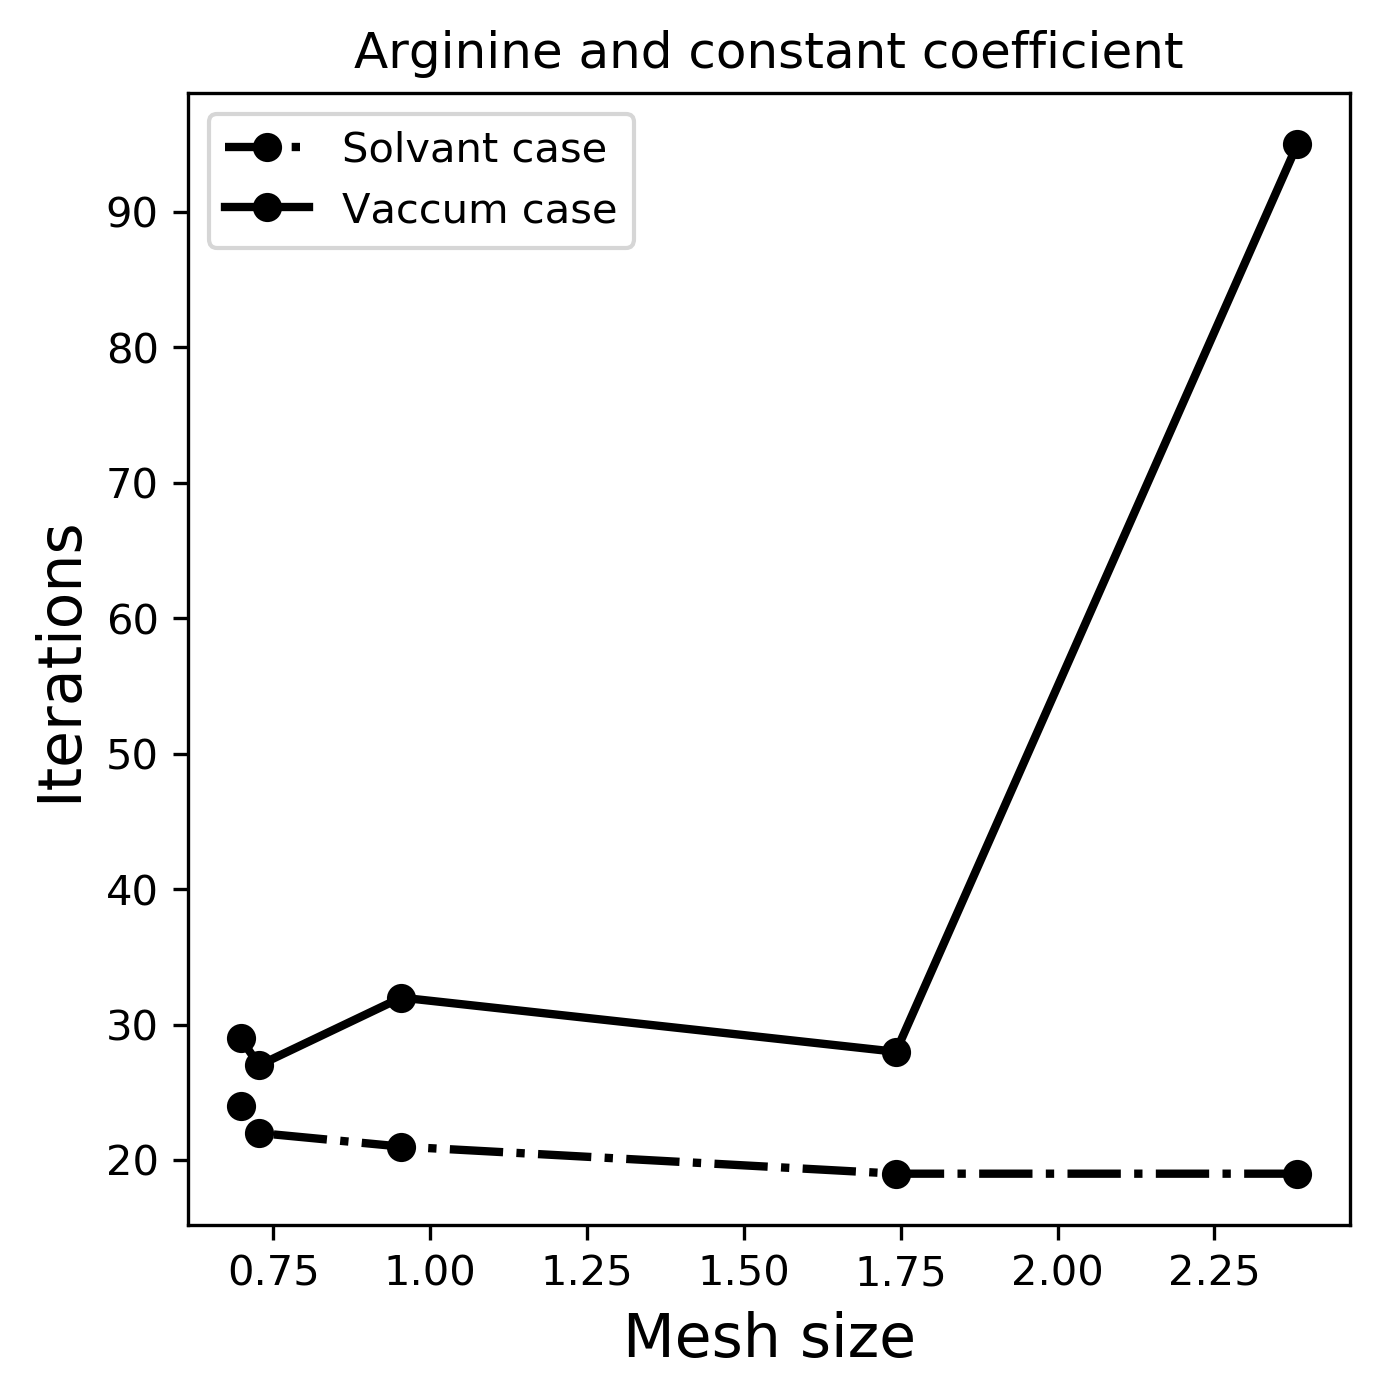
\includegraphics[width=\linewidth]{Hybrid_FEM_BEM_Arginine_const_coeff_iter.png}
  \caption{Iterations}
\endminipage\hfill
\minipage{0.45\textwidth}%
  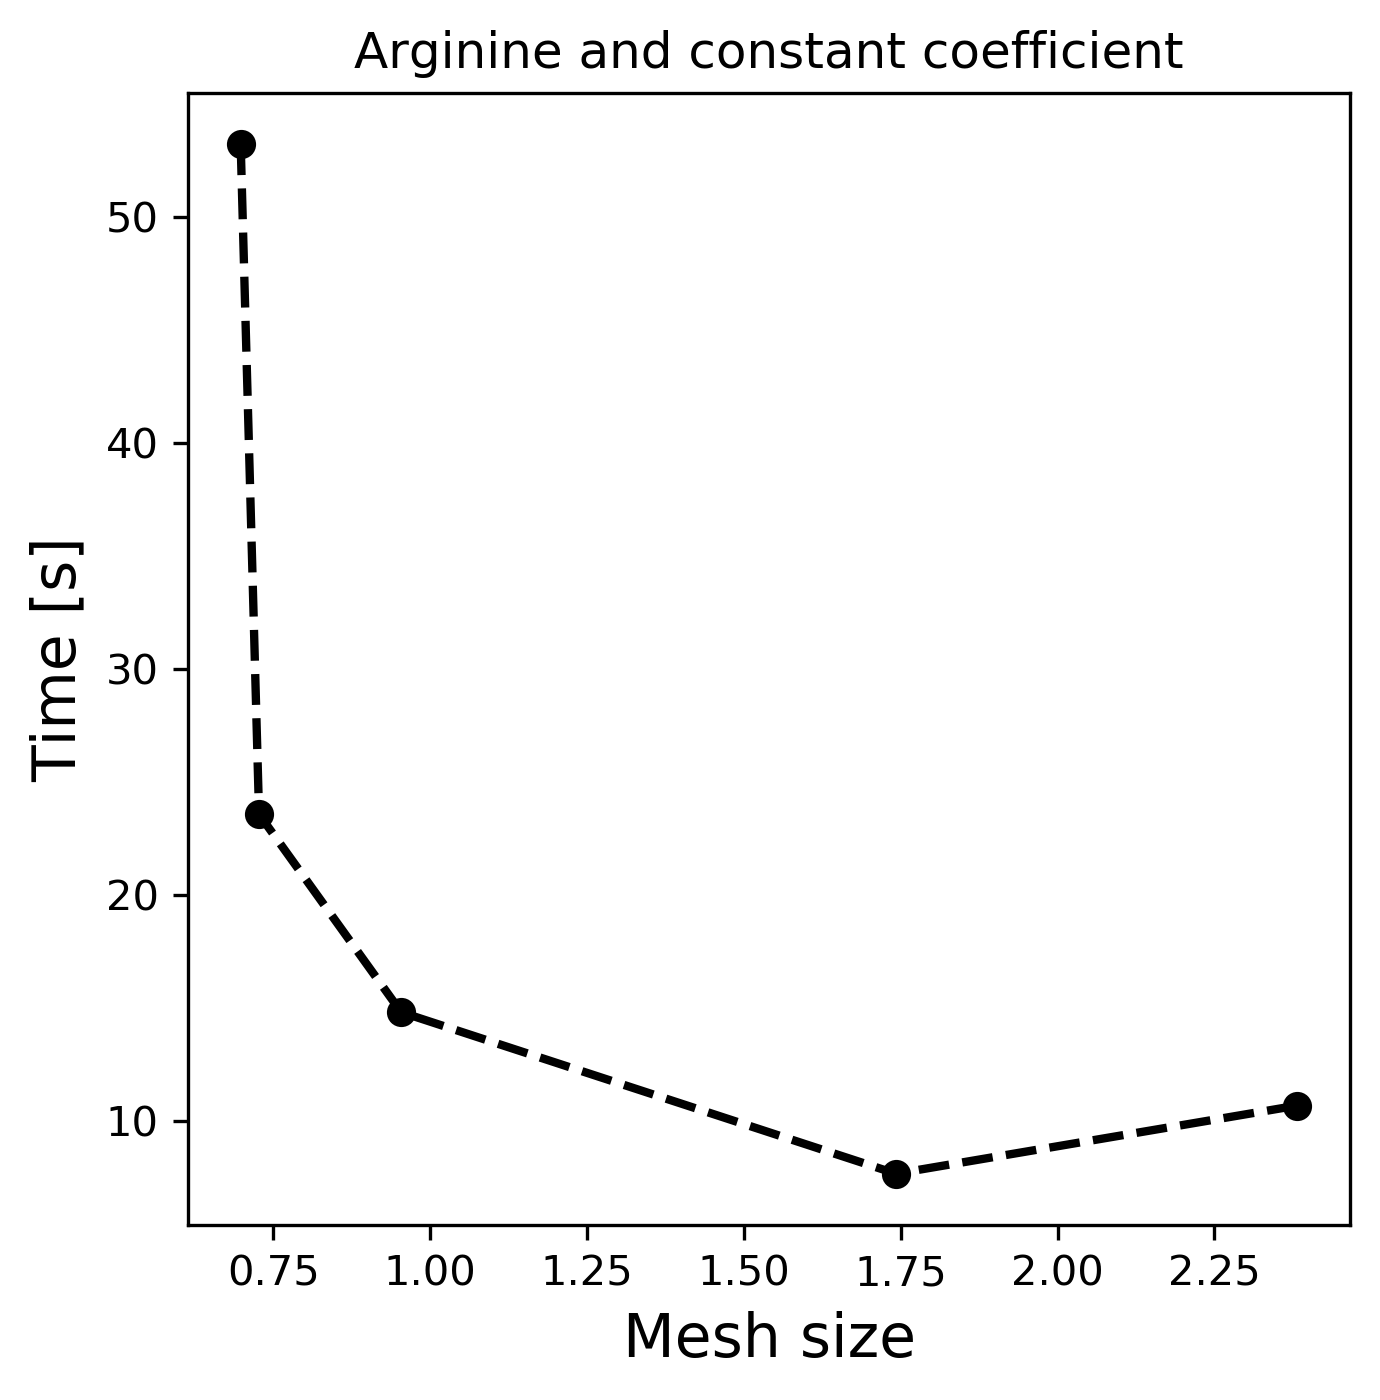
\includegraphics[width=\linewidth]{Hybrid_FEM_BEM_Arginine_const_coeff_time.png}
  \caption{Computational time}
\endminipage
\end{figure}
    \end{itemize}
    \item Compare computer time and iterations for FEM-BEM with standard and hybrid approaches, without preconditioner. Choose hybrid.
    \item Show performance of hybrid method with preconditioner.
\end{itemize}

\section*{\sffamily \Large Results with variable permittivity}

    \begin{itemize}
        \item Standard FEM-BEM
\begin{figure}[!htb]
\minipage{0.45\textwidth}
  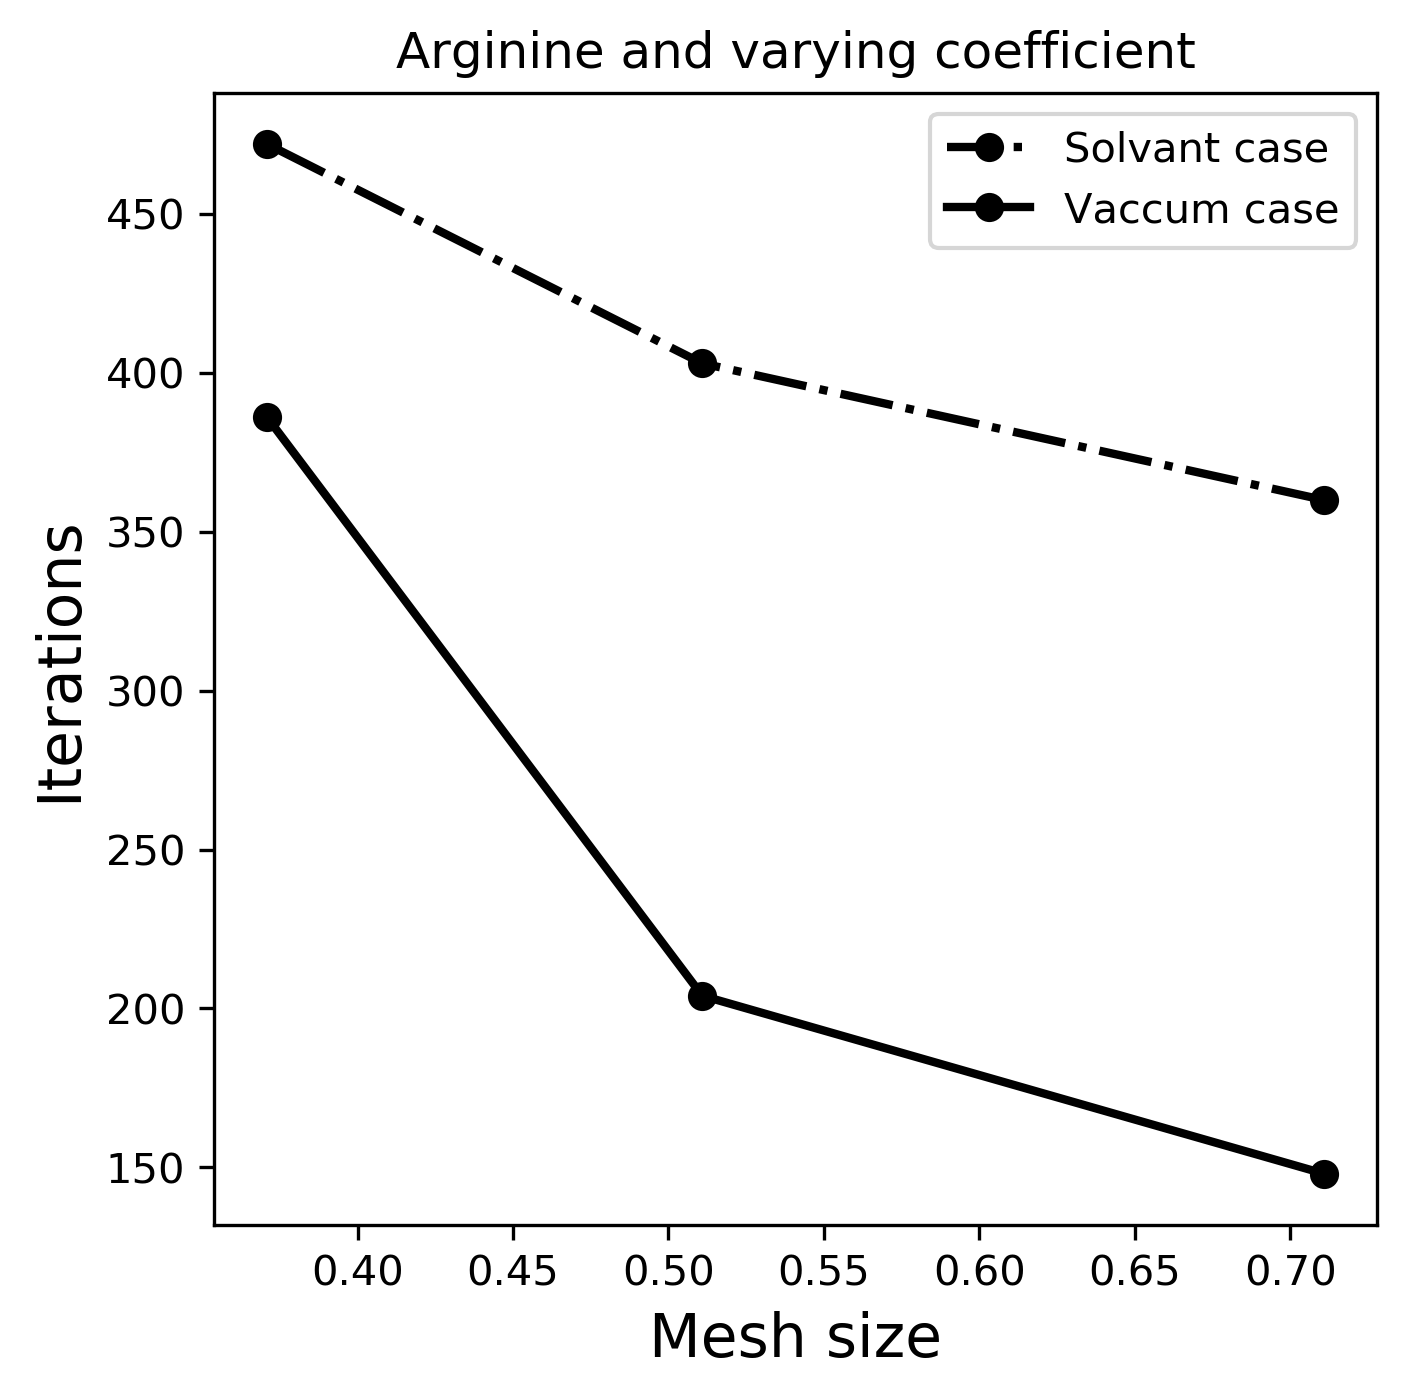
\includegraphics[width=\linewidth]{FEM_BEM_Sphere_varying_coeff_iter.png}
  \caption{Iterations}
\endminipage\hfill
\minipage{0.45\textwidth}%
  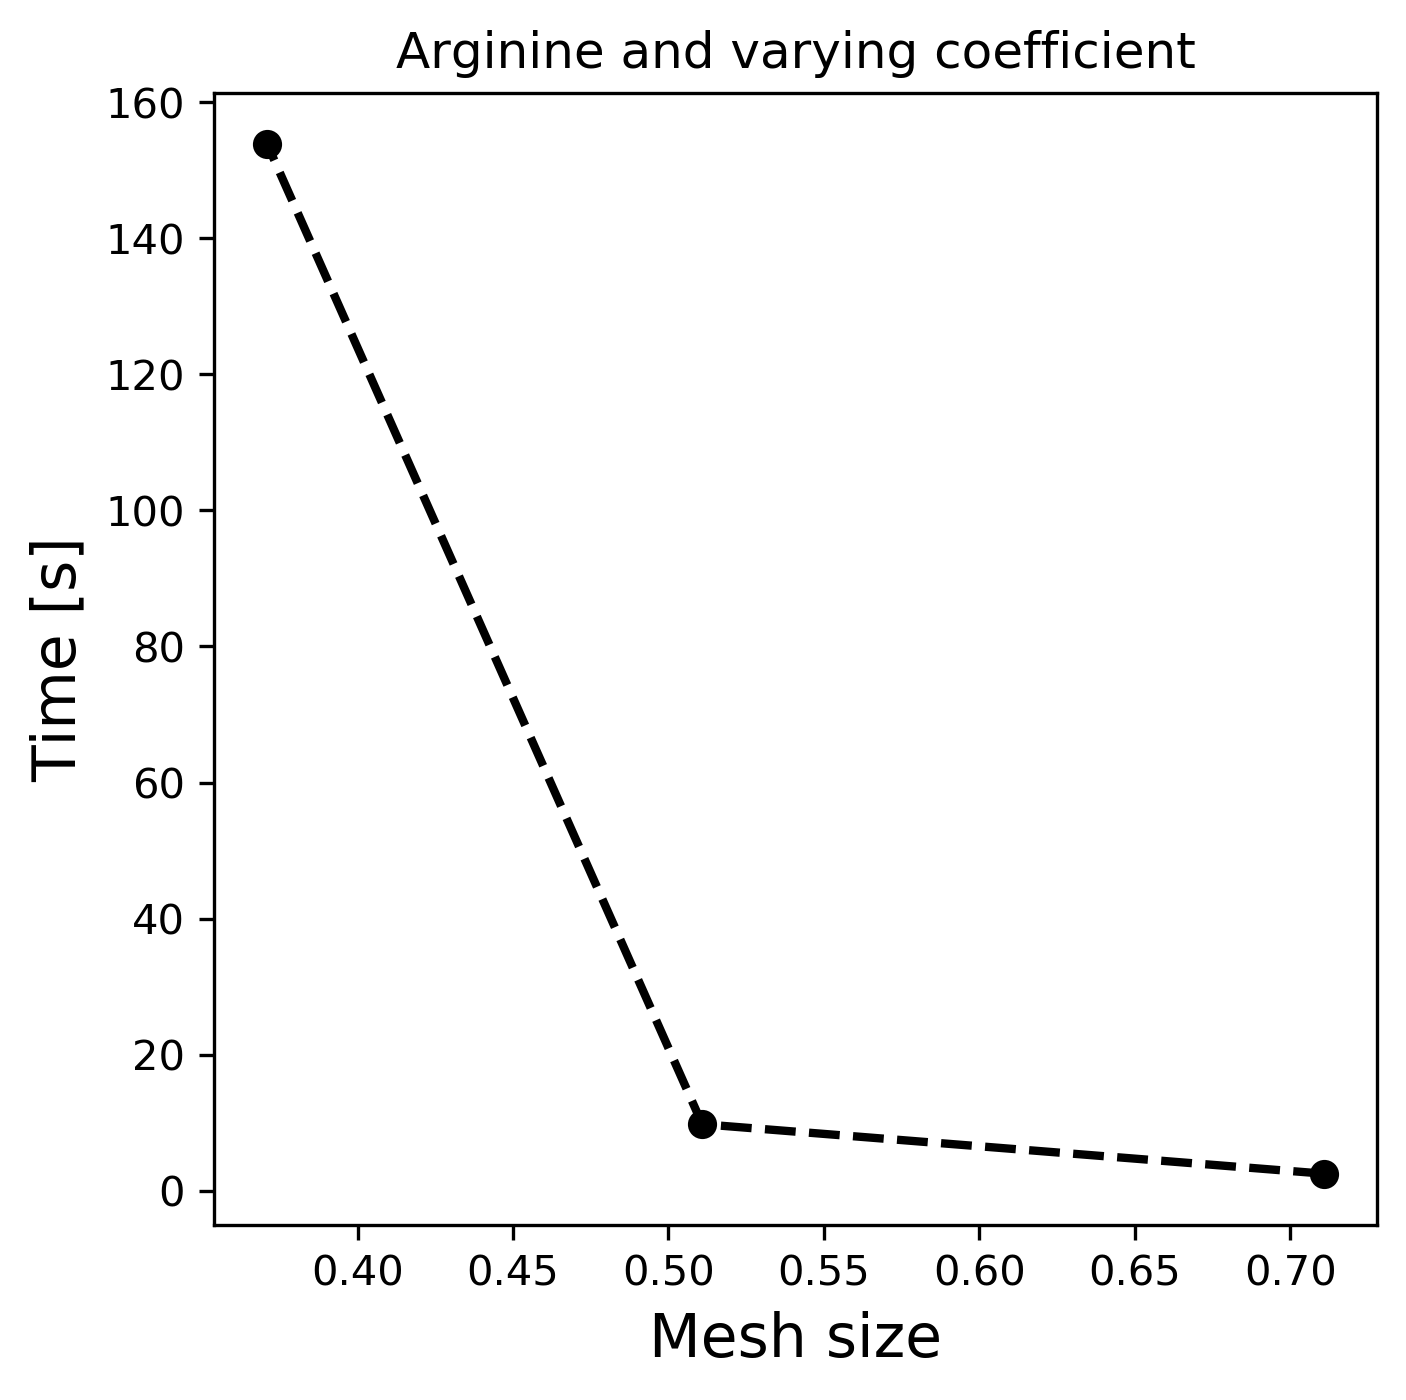
\includegraphics[width=\linewidth]{FEM_BEM_Sphere_varying_coeff_time.png}
  \caption{Computational time}
\endminipage
\end{figure}
        \item Hybrid FEM-BEM
\begin{figure}[!htb]
\minipage{0.45\textwidth}
  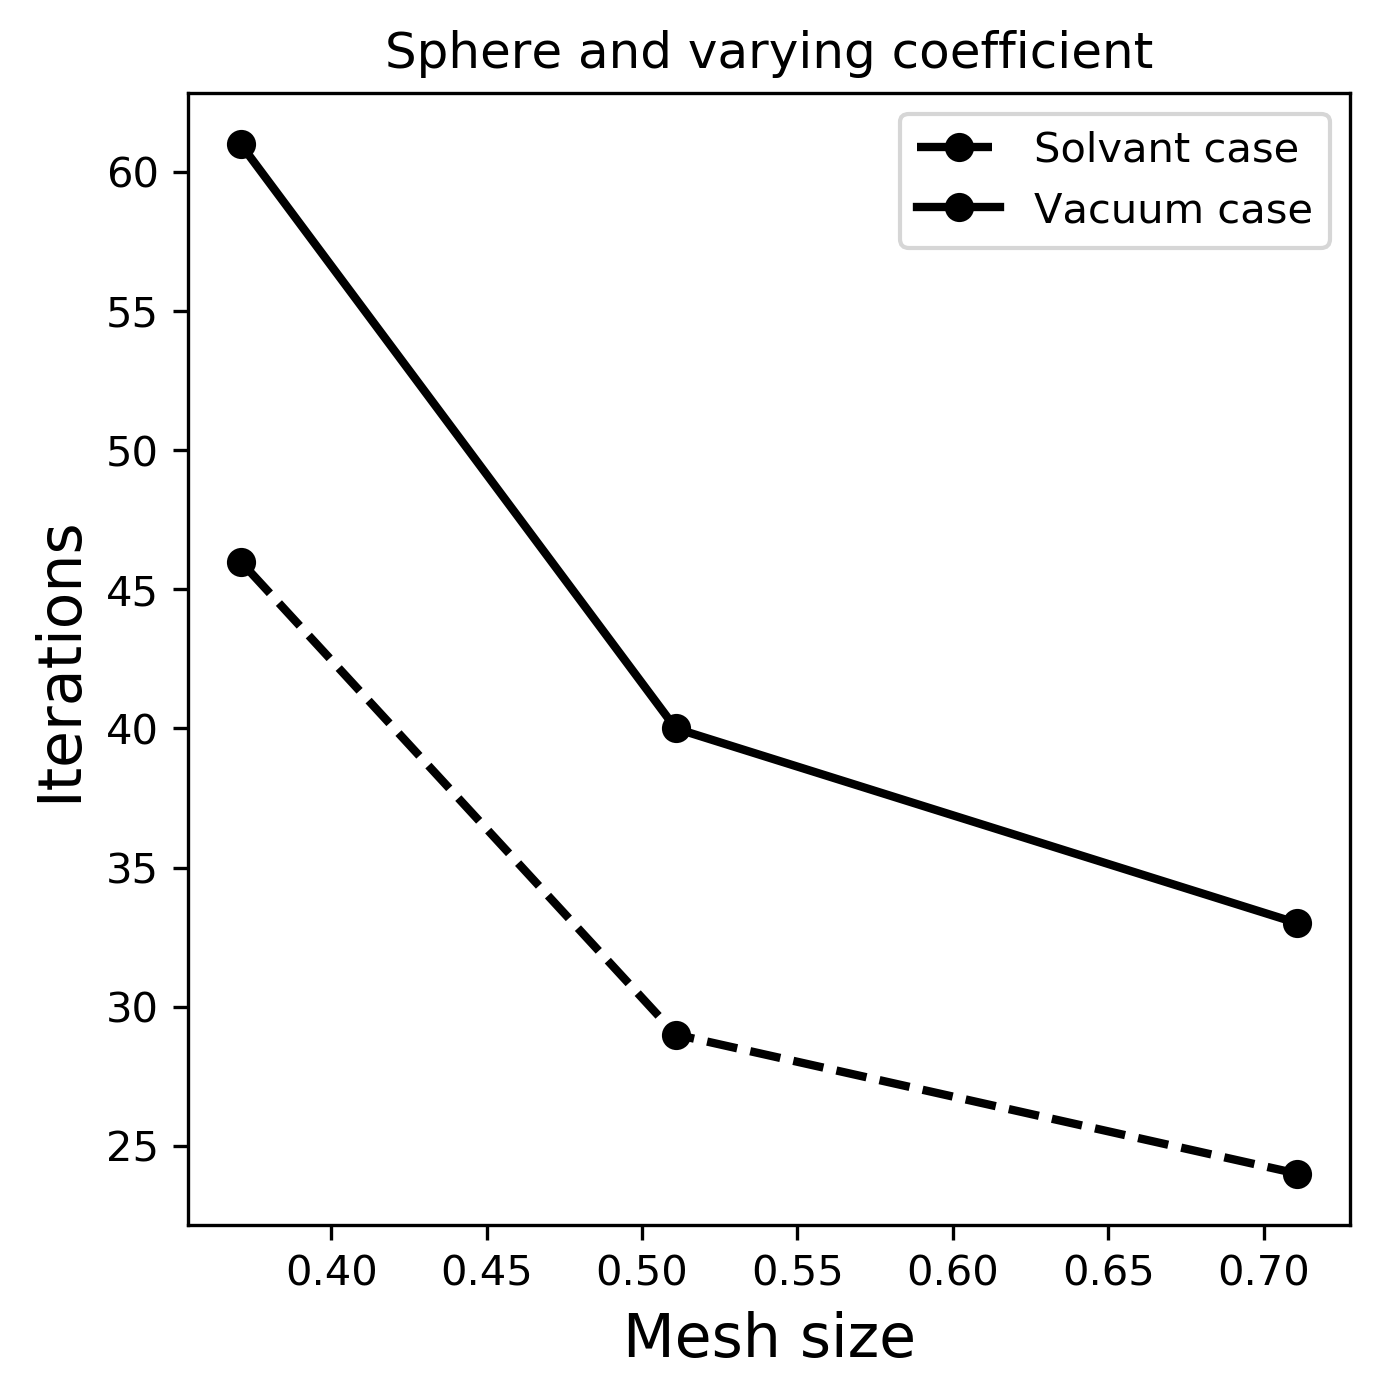
\includegraphics[width=\linewidth]{Hybrid_FEM_BEM_Sphere_varying_coeff_iter.png}
  \caption{Iterations}
\endminipage\hfill
\minipage{0.45\textwidth}%
  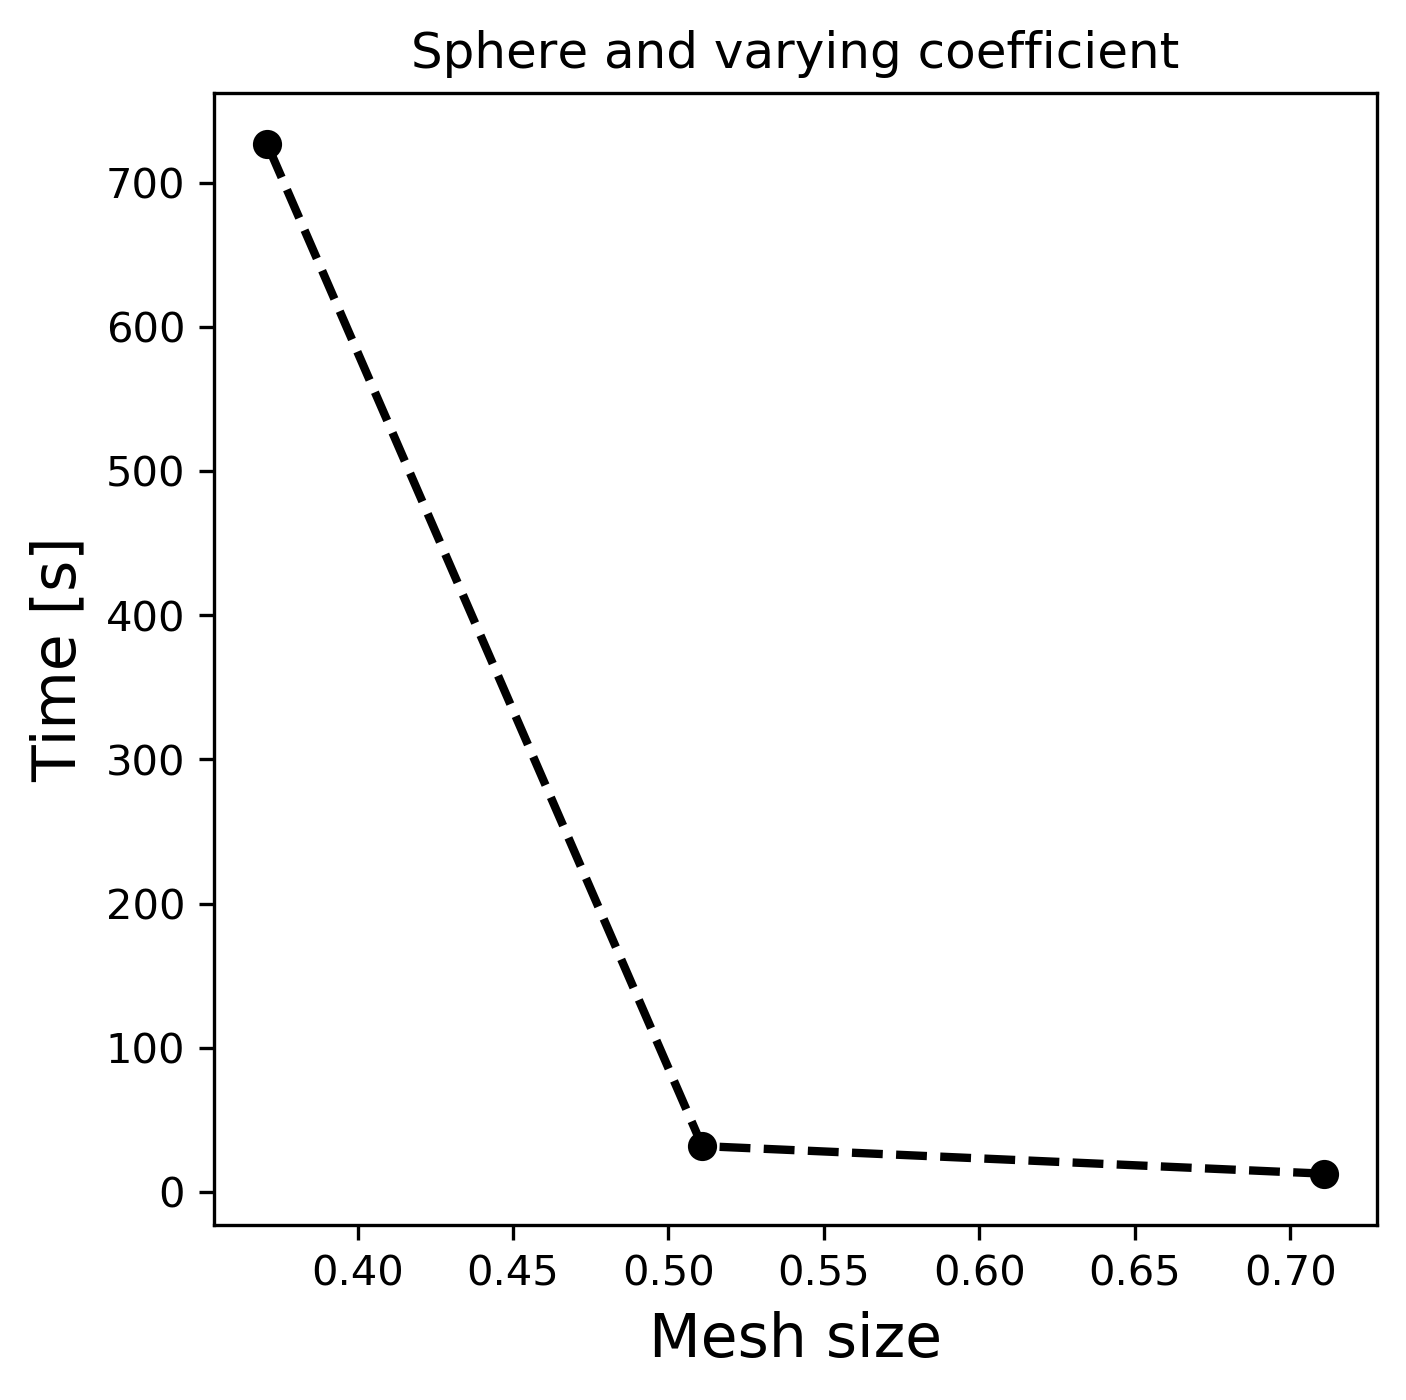
\includegraphics[width=\linewidth]{Hybrid_FEM_BEM_Sphere_varying_coeff_time.png}
  \caption{Computational time}
\endminipage
\end{figure}
    \end{itemize}

\subsection*{\sffamily \large Validation for a spherical cavity}

Compare solvation energy results of hybrid FEM-BEM with Delphi

\subsection*{\sffamily \large Convergence and performance for a molecular geometry}
\begin{itemize}
    \item Mesh refinement study using hybrid FEM-BEM and Delphi (if possible) on arginine or small protein. Check if they are converging to same result.
    \item Compare timings for equivalent error (if possible)
\end{itemize}

    \begin{itemize}
        \item Standard FEM-BEM
\begin{figure}[!htb]
\minipage{0.45\textwidth}
  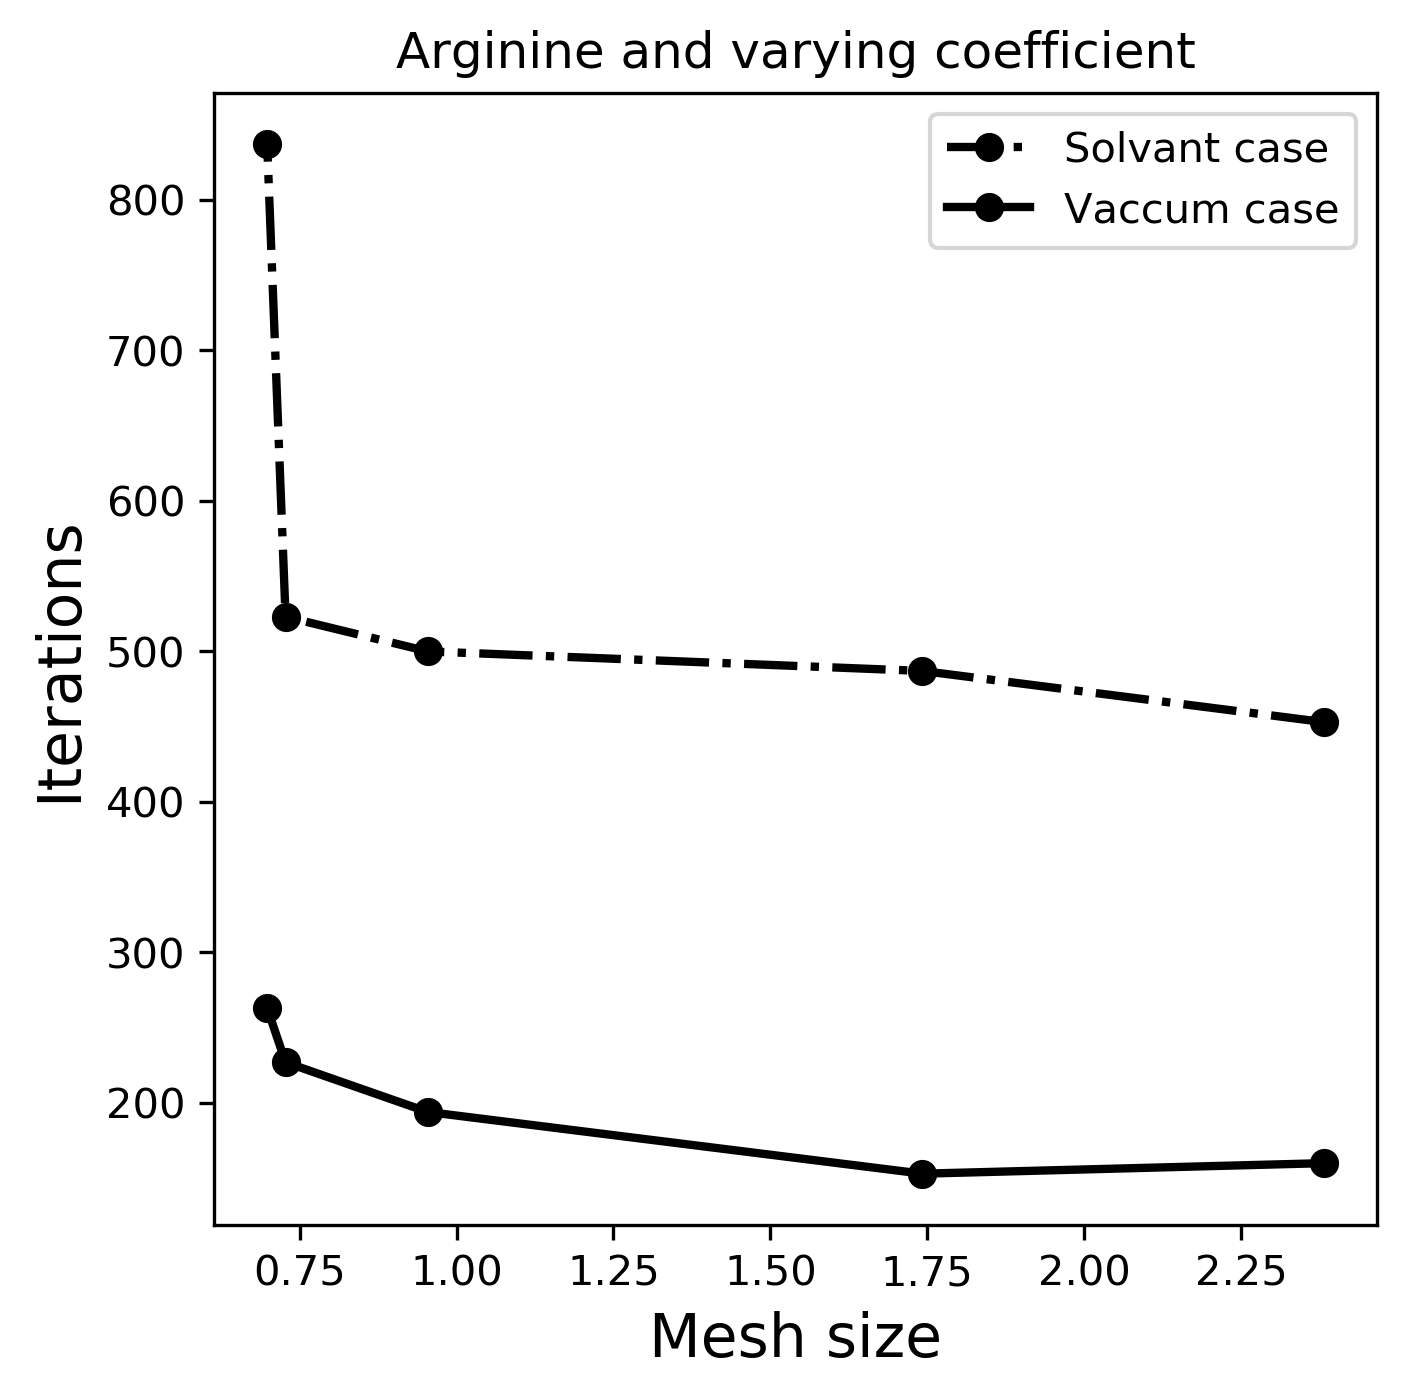
\includegraphics[width=\linewidth]{FEM_BEM_Arginine_varying_coeff_iter.png}
  \caption{Iterations}
\endminipage\hfill
\minipage{0.45\textwidth}%
  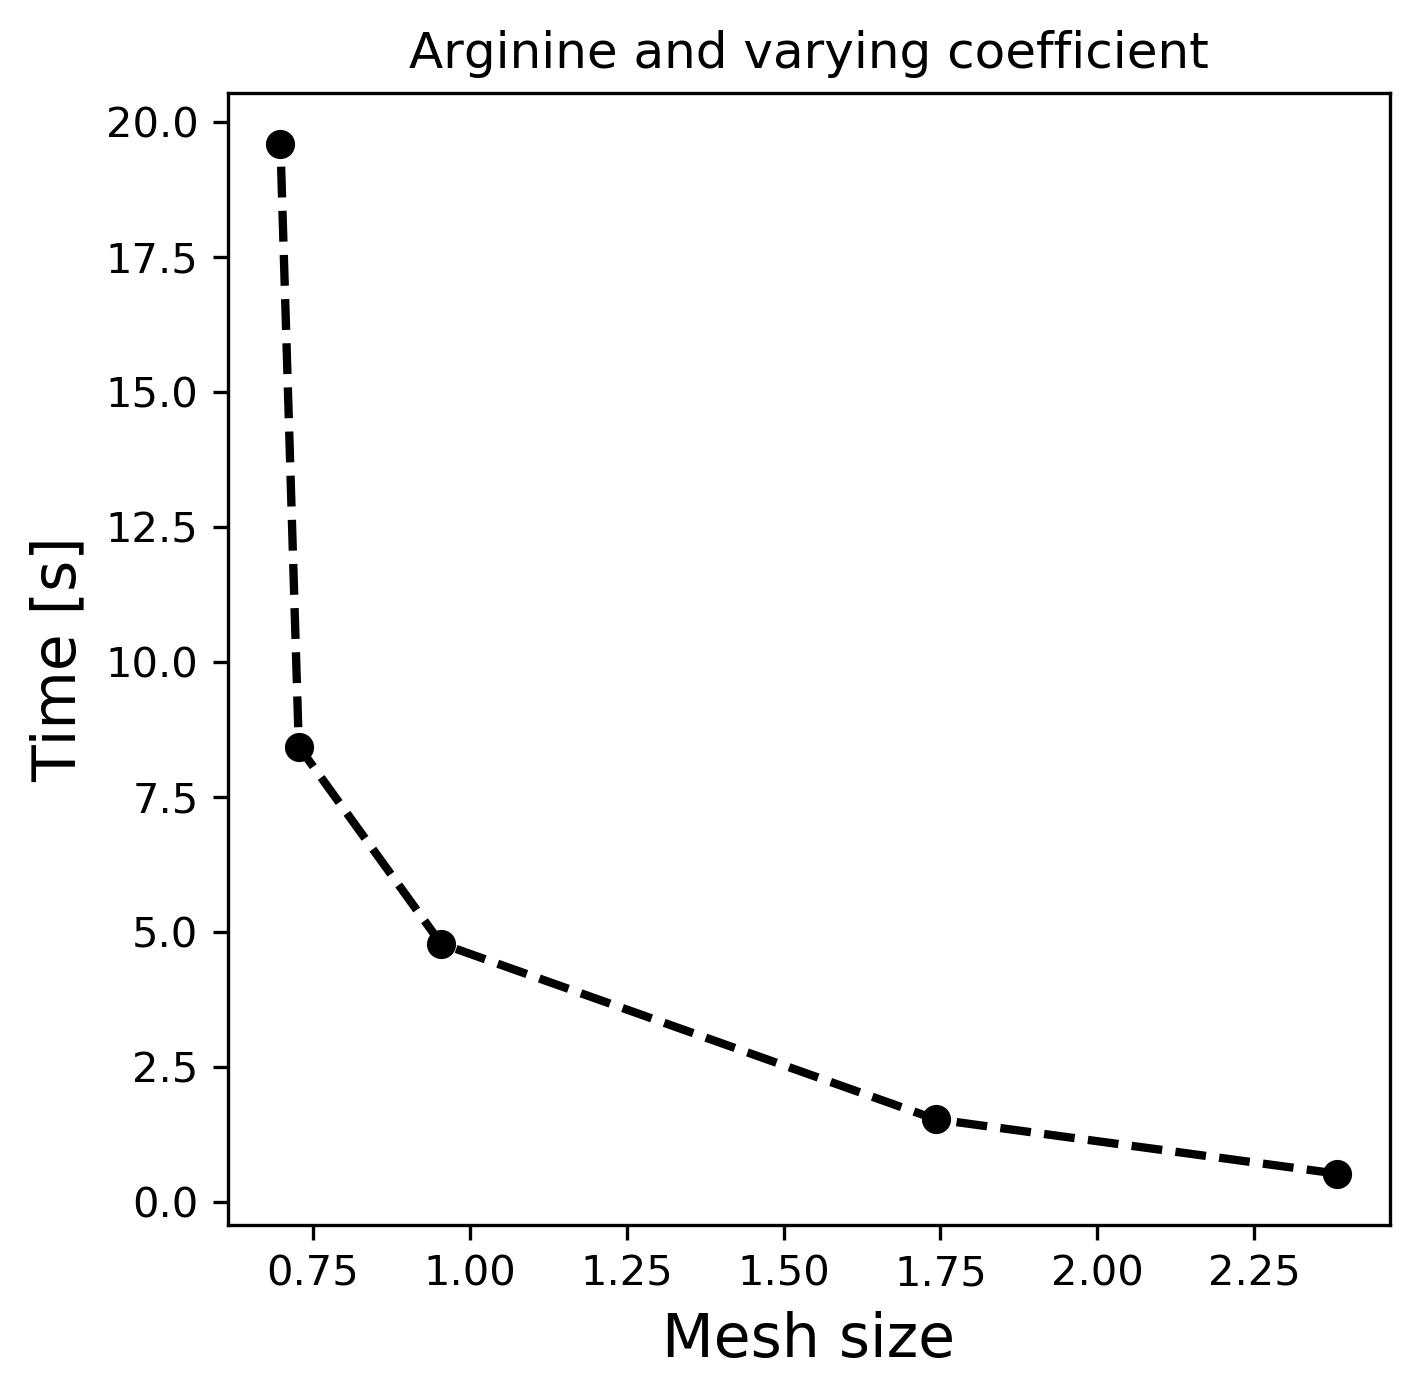
\includegraphics[width=\linewidth]{FEM_BEM_Arginine_varying_coeff_time.png}
  \caption{Computational time}
\endminipage
\end{figure}
        \item Hybrid FEM-BEM
\begin{figure}[!htb]
\minipage{0.45\textwidth}
  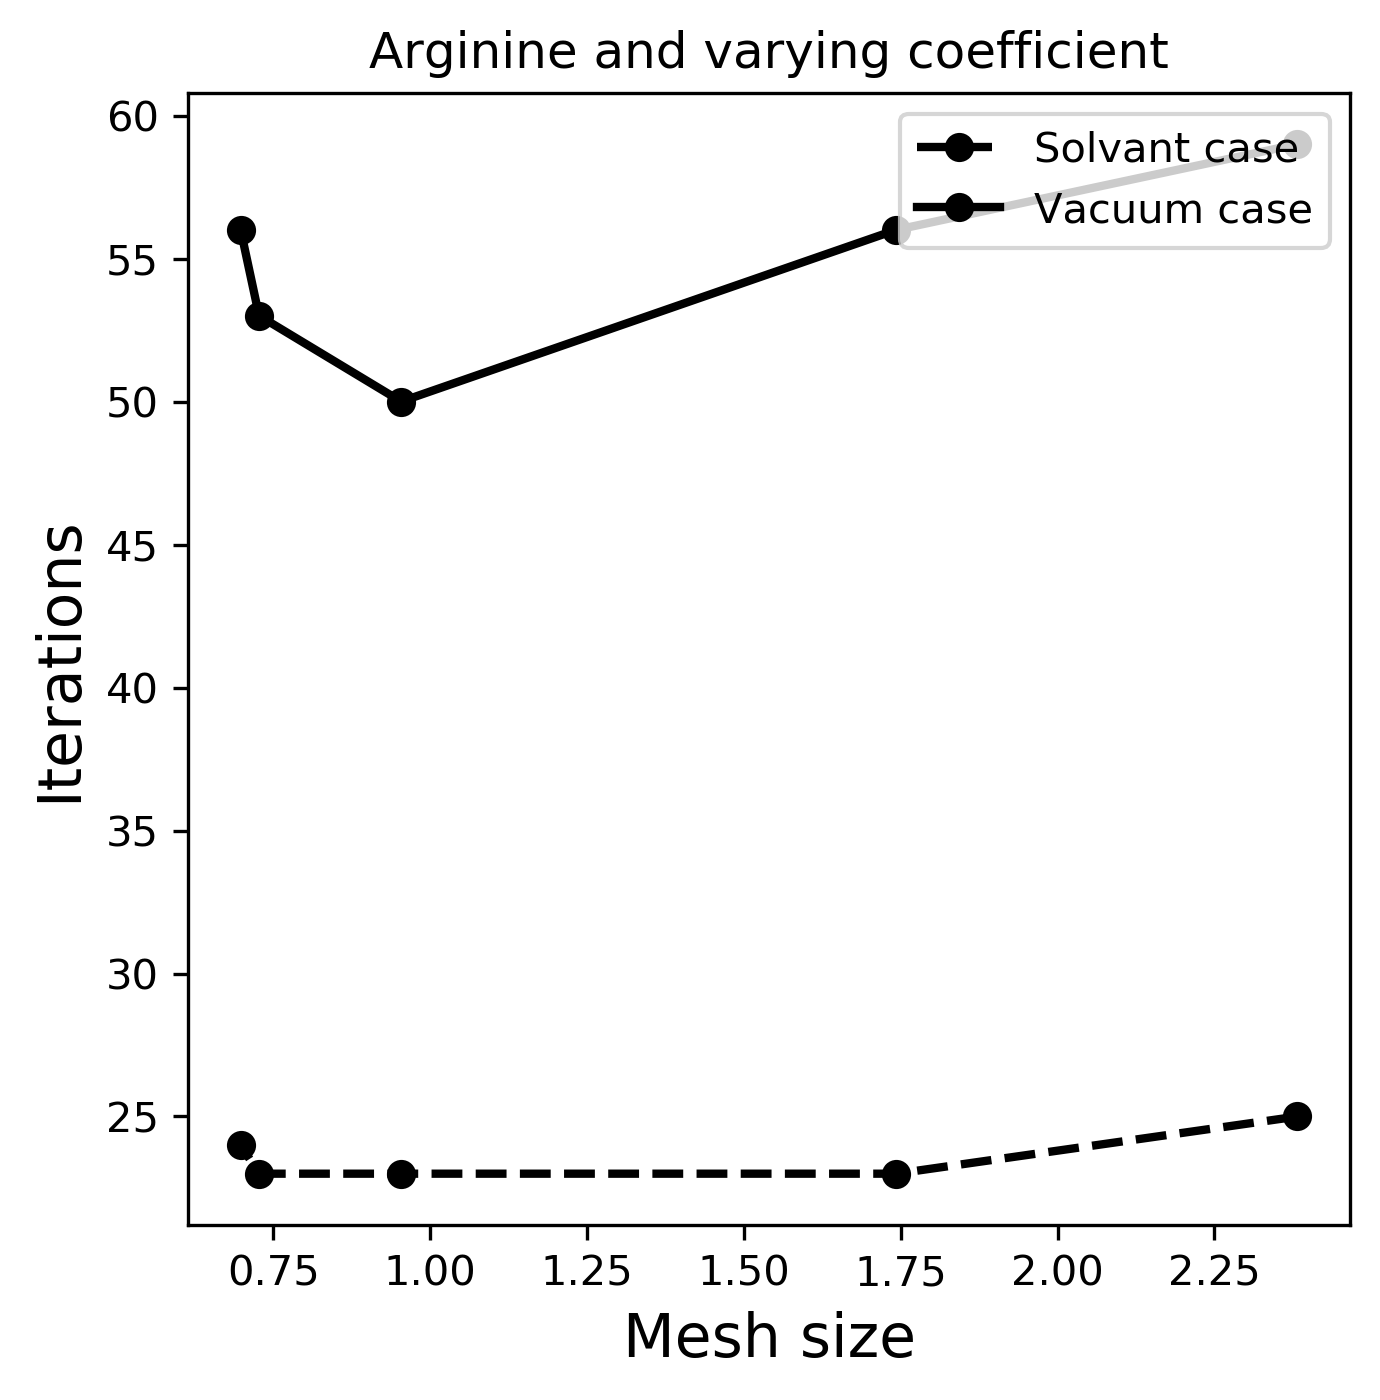
\includegraphics[width=\linewidth]{Hybrid_FEM_BEM_Arginine_varying_coeff_iter.png}
  \caption{Iterations}
\endminipage\hfill
\minipage{0.45\textwidth}%
  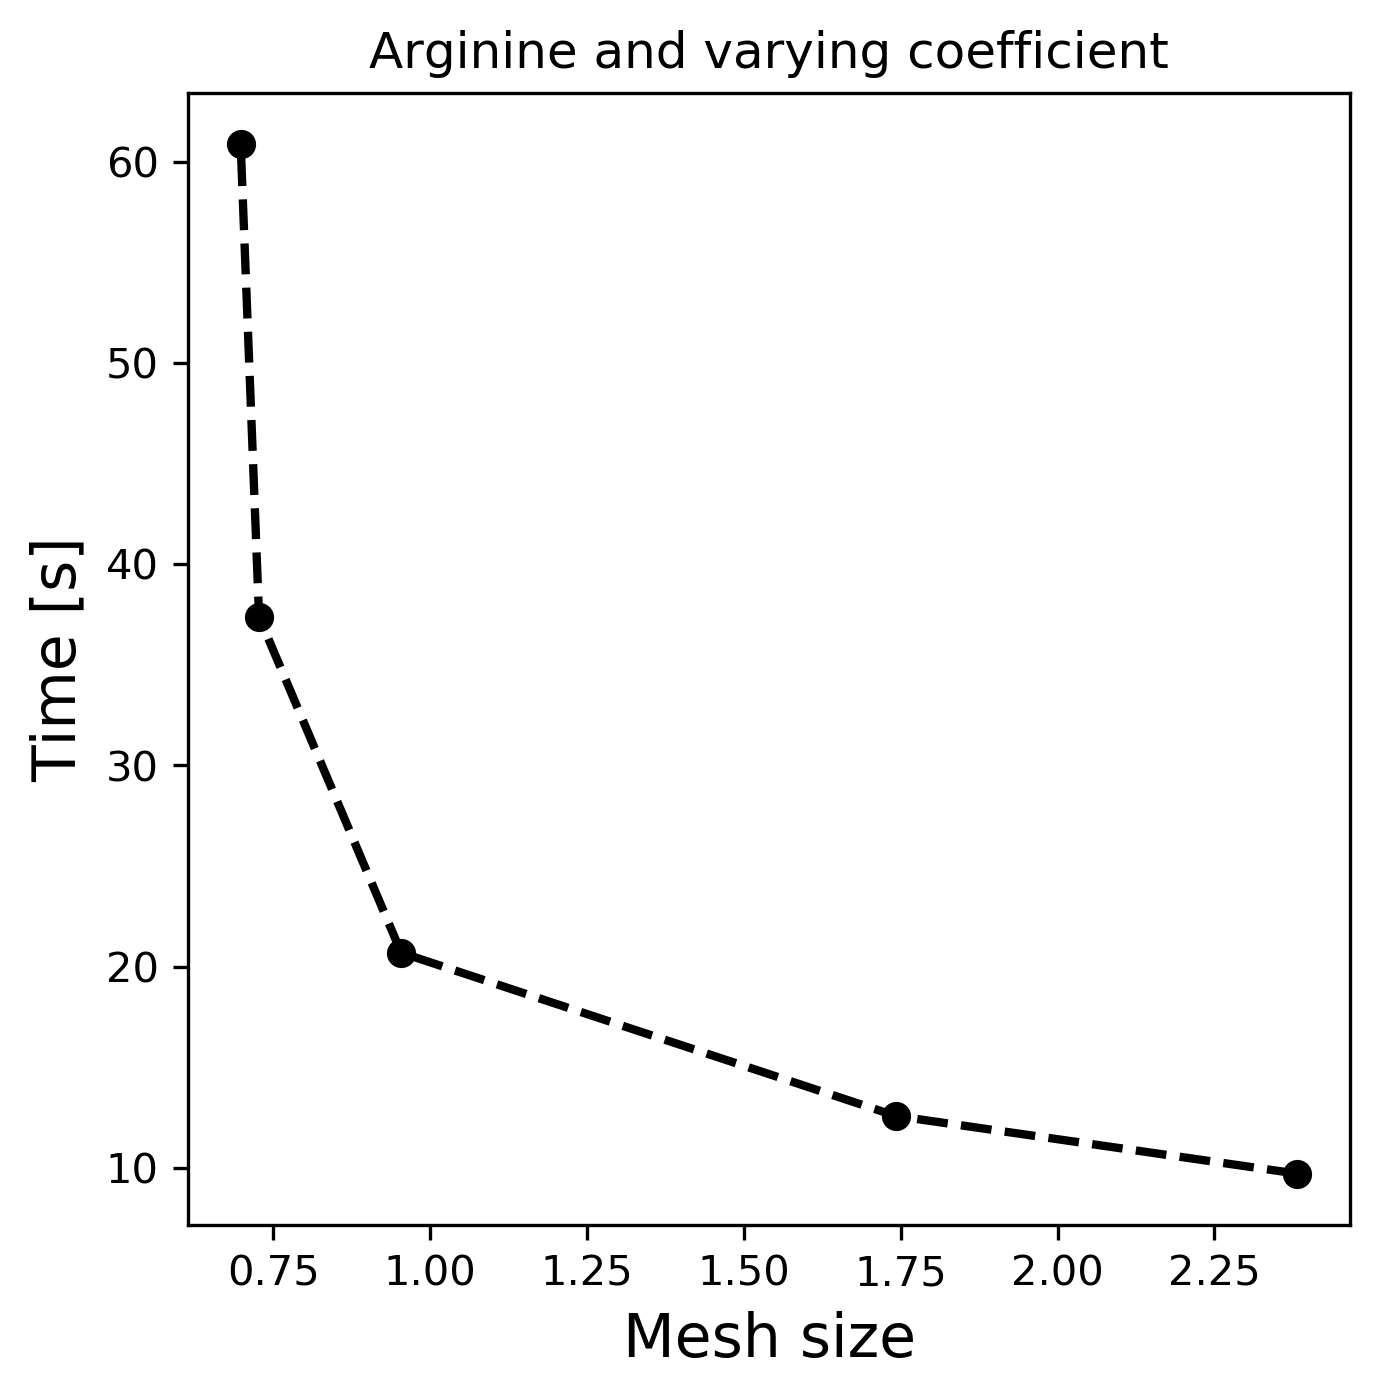
\includegraphics[width=\linewidth]{Hybrid_FEM_BEM_Arginine_varying_coeff_time.png}
  \caption{Computational time}
\endminipage
\end{figure}
    \end{itemize}

\subsection*{\sffamily \large Performance analysis for larger structures}

For a given mesh refinement, show solvation energy and timings using preconditioned hybrid FEM-BEM up to the biggest problem we can do on whatever computer we're using.
%((Place Results here. Not needed for review articles.))

\section*{\sffamily \Large First-order heading}
 
%((Equations should be inserted using standard LaTeX equation and eqnarray environments, not as graphics, and should be set in the main text))
%Equation											(1)
%((References should be superscripted and appear after punctuation.1,2 Please define all acronyms at their first usage except IR, UV, NMR, and DNA or similar commonly understood terms.)) 


\subsection*{\sffamily \large Second-order heading}

\subsubsection*{\sffamily \normalsize Third-order heading}

{\sffamily \small Fourth-order heading}\\

\section*{\sffamily \Large DISCUSSION}

%((Place Discussion here. Not needed for review articles.))


\section*{\sffamily \Large CONCLUSIONS}

%((Place Conclusions here.))

\subsection*{\sffamily \large ACKNOWLEDGMENTS}

%((Place Acknowledgments here))


%((Additional Supporting Information may be found in the online version of this article.))

\clearpage

%%%%%%%%%%%%%%%%%%%%%%%%%%%%%%%%%%%%%%%%%%%%%%%%%%%%%%%%%%%%%%%%%%%%%%%%%%%%%%%%%
% BIBLIOGRAPHY

%\bibliography{bibtexrefs}   % Produces the bibliography via BibTeX.

\begin{thebibliography}{99}


\bibitem{Coulson}
Coulson, C. A., Rev. Mod. Phys., \textbf{1960}, 32,170-177.
\bibitem{Malrieu}
Malrieu, J.-P., J. Mol. Struct., \textbf{1998}, 424, 1-2,83-91.
\bibitem{Shaik}
Shaik, S., New. J. Chem., \textbf{2007}, 31,2015-2028.
\bibitem{Hoffmann}
Hoffman, R., Schleyer, P. v. R., Schaefer III, H. F., \textbf{2008}, 47, 7164-7167.
\bibitem{Perdew}
Perdew, J. P., Ruzsinszky, A., Constantin, L., Sun, J., Csonka, G., J. Chem. Theory Comput., \textbf{2009}, 5, 902-908.
\bibitem{Koros}
Koros, W. J.; Chern, R. T. In Handbook of Separation Process Technology; Rousseau, E. D.; Russell, B., Eds.; Wiley: New York, \textbf{1987}; Vol. 2, Chapter 20, pp 34-45.
\end{thebibliography}


%%%%%%%%%%%%%%%%%%%%%%%%%%%%%%%%%%%%%%%%%%%%%%%%%%%%%%%%%%%%%%%%%%%%%%%%%%%%%%%%%

\clearpage
%%%%%%%%%%%%%%%%%%%%%%%%%%%%%%%%%%%%%%%%%%%%%%%%%%%%%%%%%%%%%%%%%%%%%%%%%%%%%%%%%
% FIGURE CAPTIONS

%%%%% FIGURE ---- cc.eps
\begin{figure}
\caption{\label{cc} Place Figure 1 caption here. In the case of reproduced figures in review articles, you must obtain the publisher's permission and state a suitable notice here along with a citation.}
\end{figure}

\begin{figure}
\caption{\label{fig2} Place Figure 2 caption here. Figures should be uploaded as individual files, preferably .tif or .eps files, at high enough resolution (600 to 1200 dpi) to ensure clarity. Please see the author’s guide for more details and specifications. For high quality illustrations, we highly recommend the use of the TikZ package.}
\end{figure}


%%%%%%%%%%%%%%%%%%%%%%%%%%%%



%%%%%%%%%%%%%%%%%%%%%%%%%%%%%%%%%%%%%%%%%%%%%%%%%%%%%%%%%%%%%%%%%%%%%%%%%%%%%%%%%
% FIGURE FILES

\clearpage

%\vspace*{0.1in}   %%% FIGURE 1
\begin{center}
\includegraphics[width=0.2\columnwidth,keepaspectratio=true]{cc.eps}
\end{center}
\vspace{0.25in}
\hspace*{3in}
{\Large
\begin{minipage}[t]{3in}
\baselineskip = .5\baselineskip
Figure 1 \\
Author A, Author B, Author C, Author D \\
J.\ Comput.\ Chem.
\end{minipage}
}

\clearpage

\begin{table}
\begin{tabular}{|c|c|c|c|}\hline
\textbf{Quantity} & \textbf{Calculated} & \textbf{Observed} & \textbf{Error} \\ \hline
  Density & 5.3 & 6.3 & Within limits \\ \hline
  Optical magnification & 8.3 & 90.9 & Utterly unacceptable\! \\ \hline
\end{tabular}
\caption{\label{tbl1} Place table caption here.}
\end{table}

\end{document}

